% !TeX document-id = {2408e792-e174-42df-a22b-01cd9180bd9b}
% !TEX TS-program = XeLaTeX
% !TeX program = xelatex
% Command for running this example (needs latexmkrc file):
%    latexmk -bibtex -pdf main.tex

%	نمونه پایان‌نامه آماده شده با استفاده از کلاس tehran-thesis، نگارش 1
%	سینا ممکن، دانشگاه تهران 
%	https://github.com/sinamomken/tehran-thesis
%	گروه پارسی‌لاتک
%	http://www.parsilatex.com
%	این نسخه، بر اساس نسخه‌ 0.1 از کلاس IUST-Thesis آقای محمود امین‌طوسی آماده شده است.
%        http://profsite.sttu.ac.ir/mamintoosi

%----------------------------------------------------------------------------------------------
% اگر قصد نوشتن پروژه کارشناسی را دارید، در خط زیر به جای msc، کلمه bsc و اگر قصد نوشتن رساله دکترا را دارید، کلمه phd را قرار دهید. کلیه تنظیمات لازم، به طور خودکار، اعمال می‌شود.



% اگر مایلید پایان‌نامه شما دورو باشد به جای oneside در خط زیر از twoside استفاده کنید.

% برای حاشیه‌نویسی و کم کردن صفحات ابتدایی، گزینه draft را وارد و برای نسخه نهایی آن را حذف کنید.

% برای استفاده از قلم‌های سری IR Series گزینه irfonts را وارد و برای استفاده از قلم‌های X Series 2 آن را حذف کنید.

\documentclass[
twoside
,openany
,bsc
,irfonts
% ,draft
]{./tex/tehran-thesis}

% فایل commands.tex را مطالعه کنید؛ چون دستورات مربوط به فراخوانی بسته‌ها، فونت و دستورات خاص در این فایل قرار دارد.
% در این فایل، دستورها و تنظیمات مورد نیاز، آورده شده است.
%-------------------------------------------------------------------------------------------------------------------
% دستوراتی که پوشه پیش‌فرض زیرفایل‌های tex را مشخص می‌کند.
%\makeatletter
%\def\input@path{{./tex/}}
%\makeatother
% در ورژن جدید زی‌پرشین برای تایپ متن‌های ریاضی، این سه بسته، حتماً باید فراخوانی شود
\usepackage{amsthm,amssymb,amsmath}
% بسته‌ای برای تنطیم حاشیه‌های بالا، پایین، چپ و راست صفحه
\usepackage[top=40mm, bottom=40mm, left=25mm, right=35mm]{geometry}
% بسته‌‌ای برای ظاهر شدن شکل‌ها و تعیین آدرس تصاویر
\usepackage[final]{graphicx}
\graphicspath{{./img/}}
% بسته‌های مورد نیاز برای نوشتن کدها، رنگ‌آمیزی آنها و تعیین پوشهٔ کدها
\usepackage[final]{listings}
\usepackage[usenames,dvipsnames,svgnames,table]{xcolor}
\lstset{inputpath=./code/}
% بسته‌ای برای رسم کادر
\usepackage{framed} 
% بسته‌‌ای برای چاپ شدن خودکار تعداد صفحات در صفحه «معرفی پایان‌نامه»
\usepackage{lastpage}
% بسته‌ٔ لازم برای: ۱. تغییر شماره‌گذاری صفحات پیوست. ۲. تصحیح باگ آدرس وب حاوی '%' در مراجع
\usepackage{etoolbox}

%%%%%%%%%%%%%%%%%%%%%%%%%%%%%%%%%%%%
%%% دستورات وابسته به استیل مراجع:
%% اگر از استیل‌های natbib (plainnat-fa، asa-fa، chicago-fa) استفاده می‌کنید، خط زیر را فعال و بعدی‌اش را غیرفعال کنید.
%\usepackage{natbib}
%\newcommand{\citelatin}[1]{\cite{#1}\LTRfootnote{\citeauthor*{#1}}}
%\newcommand{\citeplatin}[1]{\citep{#1}\LTRfootnote{\citeauthor*{#1}}}
%% اگر از سایر استیل‌ها استفاده می‌کنید، خط بالا را غیرفعال و خط‌های زیر را فعال کنید.
\let\citep\cite
\let\citelatin\cite
\let\citeplatin\cite
%%%%%%%%%%%%
% بررسی حالت پیش نویس
\usepackage{ifdraft}
\ifdraft
{%
	% بسته‌ٔ ایجاد لینک‌های رنگی با امکان جهش
	\usepackage[unicode=true,pagebackref=true,
colorlinks,linkcolor=blue,citecolor=blue,final]{hyperref}
	%\usepackage{todonotes}
	\usepackage[firstpage]{draftwatermark}
	\SetWatermarkText{\ \ \ پیش‌نویس}
	\SetWatermarkScale{1.2}
}
{ 
	\usepackage[pagebackref=false,colorlinks,
	linkcolor=blue,citecolor=blue,urlcolor=blue]{hyperref}
	%\usepackage[disable]{todonotes} % final without TODOs
}

\usepackage[obeyDraft]{todonotes}
\setlength{\marginparwidth}{2cm}

%%%%%%%%%%%%
%%% تصحیح باگ: اگر در مراجع، آدرس وب حاوی '%' بوده و pagebackref فعال باشد، دستورات زیر باید بیایند:
%% برای استیل‌های natbib مثل plainnat-fa، asa-fa، chicago-fa
\makeatletter
\let\ORIG@BR@@lbibitem\BR@@lbibitem
\apptocmd\ORIG@BR@@lbibitem{\endgroup}{}{}
\def\BR@@lbibitem{\begingroup\catcode`\%=12 \ORIG@BR@@lbibitem}
\makeatother
%% برای سایر استیل‌ها
\makeatletter
\let\ORIG@BR@@bibitem\BR@@bibitem
\apptocmd\ORIG@BR@@bibitem{\endgroup}{}{}
\def\BR@@bibitem{\begingroup\catcode`\%=12 \ORIG@BR@@bibitem}
\makeatother
%%%%%%%%%%%%%%%%%%%%%%%%%%%%%%%%%%%%

% بسته‌ لازم برای تنظیم سربرگ‌ها
\usepackage{fancyhdr}
%\usepackage{enumitem}
\usepackage{setspace}
% بسته‌های لازم برای نوشتن الگوریتم
\usepackage{algorithm}
\usepackage{algorithmic}
% بسته‌های لازم برای رسم بهتر جداول
\usepackage{tabulary}
\usepackage{tabularx}
\usepackage{rotating}
% بسته‌های لازم برای رسم تنظیم بهتر شکل‌ها و زیرشکل‌ها
\usepackage[export]{adjustbox}
\usepackage{subfig}
\usepackage[subfigure]{tocloft}
% بسته‌ای برای رسم نمودارها و نیز صفحه مالکیت اثر
\usepackage{tikz}
% بسته‌ای برای ظاهر شدن «مراجع» و «نمایه» در فهرست مطالب
\usepackage[nottoc]{tocbibind}
% دستورات مربوط به ایجاد نمایه
\usepackage{makeidx}
\makeindex
%%% بسته ایجاد واژه‌نامه با xindy
\usepackage[xindy,acronym,nonumberlist=true]{glossaries}

% بسته زیر باگ ناشی از فراخوانی بسته‌های زیاد را برطرف می‌کند.
\usepackage{morewrites}
%%%%%%%%%%%%%%%%%%%%%%%%%%
% فراخوانی بسته زی‌پرشین (باید آخرین بسته باشد)
\usepackage[extrafootnotefeatures, localise=on, displaymathdigits=persian]{xepersian}




\makeatletter
% تعریف قلم فارسی و انگلیسی و مکان قلم‌ها
\if@irfonts
\settextfont[Path={./font/}, BoldFont={IRLotusICEE_Bold.ttf}, BoldItalicFont={IRLotusICEE_BoldIranic.ttf}, ItalicFont={IRLotusICEE_Iranic.ttf},Scale=1.2]{IRLotusICEE.ttf}
% LiberationSerif or FreeSerif as free equivalents of Times New Roman
\setlatintextfont[Path={./font/}, BoldFont={LiberationSerif-Bold.ttf}, BoldItalicFont={LiberationSerif-BoldItalic.ttf}, ItalicFont={LiberationSerif-Italic.ttf},Scale=1]{LiberationSerif-Regular.ttf}
% چنانچه می‌خواهید اعداد در فرمول‌ها، انگلیسی باشد، خط زیر را غیرفعال کنید
% و گزینهٔ displaymathdigits=persian را از خط ۱۰۹ حذف کنید.
\setdigitfont[Path={./font/}, Scale=1.2]{IRLotusICEE.ttf}
% تعریف قلم‌های فارسی و انگلیسی اضافی برای استفاده در بعضی از قسمت‌های متن
\setiranicfont[Path={./font/}, Scale=1.3]{IRLotusICEE_Iranic.ttf}				% ایرانیک، خوابیده به چپ
\setmathsfdigitfont[Path={./font/}]{IRTitr.ttf}
\defpersianfont\titlefont[Path={./font/}, Scale=1]{IRTitr.ttf}
% برای تعریف یک قلم خاص عنوان لاتین، خط بعد را فعال و ویرایش کنید و خط بعد از آن را غیرفعال کنید.
% \deflatinfont\latintitlefont[Scale=1]{LiberationSerif}
\font\latintitlefont=cmssbx10 scaled 2300 %cmssbx10 scaled 2300
\else
\settextfont{XB Niloofar}
\setlatintextfont{Junicode}
% چنانچه می‌خواهید اعداد در فرمول‌ها، انگلیسی باشد، خط زیر را غیرفعال کنید
% و گزینهٔ displaymathdigits=persian را از خط ۱۰۹ حذف کنید.
\setdigitfont{XB Niloofar}
% تعریف قلم‌های فارسی و انگلیسی اضافی برای استفاده در بعضی از قسمت‌های متن
% \setmathsfdigitfont{XB Titre}
\defpersianfont\titlefont{XB Titre}
\deflatinfont\latintitlefont[Scale=1.1]{Junicode}
\fi
\makeatother

% برای استفاده از قلم نستعلیق خط بعد را فعال کنید.
% \defpersianfont\nastaliq[Scale=1.2]{IranNastaliq}


%%%%%%%%%%%%%%%%%%%%%%%%%%
% راستچین شدن todonotes
\presetkeys{todonotes}{align=right,textdirection=righttoleft}{}
\makeatletter
\providecommand\@dotsep{5}
\def\listtodoname{فهرست کارهای باقیمانده}
\def\listoftodos{\noindent{\Large\vspace{10mm}\textbf{\listtodoname}}\@starttoc{tdo}}
\renewcommand{\@todonotes@MissingFigureText}{شکل}
\renewcommand{\@todonotes@MissingFigureUp}{شکل}
\renewcommand{\@todonotes@MissingFigureDown}{جاافتاده}
\makeatother
% دستوری برای حذف کلمه «چکیده»
\renewcommand{\abstractname}{}
% دستوری برای حذف کلمه «abstract»
%\renewcommand{\latinabstract}{}
% دستوری برای تغییر نام کلمه «اثبات» به «برهان»
\renewcommand\proofname{\textbf{برهان}}
% دستوری برای تغییر نام کلمه «کتاب‌نامه» به «مراجع»
\renewcommand{\bibname}{مراجع}
% دستوری برای تعریف واژه‌نامه انگلیسی به فارسی
\newcommand\persiangloss[2]{#1\dotfill\lr{#2}\\}
% دستوری برای تعریف واژه‌نامه فارسی به انگلیسی 
\newcommand\englishgloss[2]{#2\dotfill\lr{#1}\\}
% تعریف دستور جدید «\پ» برای خلاصه‌نویسی جهت نوشتن عبارت «پروژه/پایان‌نامه/رساله»
\newcommand{\پ}{پروژه/پایان‌نامه/رساله }

%\newcommand\BackSlash{\char`\\}

%%%%%%%%%%%%%%%%%%%%%%%%%%
% \SepMark{-}

% تعریف و نحوه ظاهر شدن عنوان قضیه‌ها، تعریف‌ها، مثال‌ها و ...
\theoremstyle{definition}
\newtheorem{definition}{تعریف}[section]
\theoremstyle{theorem}
\newtheorem{theorem}[definition]{قضیه}
\newtheorem{lemma}[definition]{لم}
\newtheorem{proposition}[definition]{گزاره}
\newtheorem{corollary}[definition]{نتیجه}
\newtheorem{remark}[definition]{ملاحظه}
\theoremstyle{definition}
\newtheorem{example}[definition]{مثال}

%\renewcommand{\theequation}{\thechapter-\arabic{equation}}
%\def\bibname{مراجع}
\numberwithin{algorithm}{chapter}
\def\listalgorithmname{فهرست الگوریتم‌ها}
\def\listfigurename{فهرست تصاویر}
\def\listtablename{فهرست جداول}

%%%%%%%%%%%%%%%%%%%%%%%%%%%%
%%% دستورهایی برای سفارشی کردن سربرگ صفحات:
%\newcommand{\SetHeader}[1]{
% دستور زیر معادل با گزینه twoside است.
%\csname@twosidetrue\endcsname
\pagestyle{fancy}
%% دستورات زیر سبک صفحات fancy را تغییر می‌دهد:
% O=Odd, E=Even, L=Left, R=Right
% در صورت oneside بودن، عنوان فصل، سمت چپ ظاهر می‌شود.
\fancyhead{}
\fancyhead[OL]{\small\leftmark}
\fancyhead[ER]{\small\leftmark}
\fancyhead[OR]{\footnotesize\rightmark}
\fancyhead[EL]{\footnotesize\rightmark}
\renewcommand{\headrulewidth}{0.75pt}
% شکل‌دهی شماره و عنوان فصل در سربرگ
\renewcommand{\chaptermark}[1]{\markboth{فصل~\thechapter:\ #1}{}}
\makeatletter
\renewcommand{\rightmark}[1]{\@title}
\makeatother
%}
%%%%%%%%%%%%%%%%%%%%%%%%%%%%
%\def\MATtextbaseline{1.5}
%\renewcommand{\baselinestretch}{\MATtextbaseline}
\doublespacing
%%%%%%%%%%%%%%%%%%%%%%%%%%%%%
% دستوراتی برای اضافه کردن کلمه «فصل» در فهرست مطالب

\newlength\mylenprt
\newlength\mylenchp
\newlength\mylenapp

\renewcommand\cftpartpresnum{\partname~}
\renewcommand\cftchappresnum{\chaptername~}
\renewcommand\cftchapaftersnum{:}

\settowidth\mylenprt{\cftpartfont\cftpartpresnum\cftpartaftersnum}
\settowidth\mylenchp{\cftchapfont\cftchappresnum\cftchapaftersnum}
\settowidth\mylenapp{\cftchapfont\appendixname~\cftchapaftersnum}
\addtolength\mylenprt{\cftpartnumwidth}
\addtolength\mylenchp{\cftchapnumwidth}
\addtolength\mylenapp{\cftchapnumwidth}

\setlength\cftpartnumwidth{\mylenprt}
\setlength\cftchapnumwidth{\mylenchp}	

\makeatletter
{\def\thebibliography#1{\chapter*{\refname\@mkboth
   {\uppercase{\refname}}{\uppercase{\refname}}}\list
   {[\arabic{enumi}]}{\settowidth\labelwidth{[#1]}
   \rightmargin\labelwidth
   \advance\rightmargin\labelsep
   \advance\rightmargin\bibindent
   \itemindent -\bibindent

   \listparindent \itemindent
   \parsep \z@
   \usecounter{enumi}}
   \def\newblock{}
   \sloppy
   \sfcode`\.=1000\relax}}
   
%اگر مایلید در شماره گذاری حرفی و ابجد به جای آ از الف استفاده شود دستورات زیر را فعال کنید.   
%\def\@Abjad#1{%
%  \ifcase#1\or الف\or ب\or ج\or د%
%           \or هـ\or و\or ز\or ح\or ط%
%           \or ی\or ک\or ل\or م\or ن%
%           \or س\or ع\or ف\or ص%
%           \or ق\or ر\or ش\or ت\or ث%
%            \or خ\or ذ\or ض\or ظ\or غ%
%            \else\@ctrerr\fi}
%
% \def\abj@num@i#1{%
%   \ifcase#1\or الف\or ب\or ج\or د%
%            \or هـ‍\or و\or ز\or ح\or ط\fi

%   \ifnum#1=\z@\abjad@zero\fi}   
%  
%   \def\@harfi#1{\ifcase#1\or الف\or ب\or پ\or ت\or ث\or

% ج\or چ\or ح\or خ\or د\or ذ\or ر\or ز\or ژ\or س\or ش\or ص\or ض\or ط\or ظ\or ع\or غ\or

% ف\or ق\or ک\or گ\or ل\or م\or ن\or و\or ه\or ی\else\@ctrerr\fi}

%
\makeatother

%%% امکان درج کد در سند
% در این قسمت رنگ، قلم و قالب‌بندی قسمت‌های مختلف یک کد تعیین می‌شود. 
\lstdefinestyle{myStyle}{
	basicstyle=\ttfamily, % whole listing /w verbatim font
	keywordstyle=\color{blue}\bfseries, % bold black keywords
	identifierstyle=, % nothing happens
	commentstyle=\color{LimeGreen}, % green comments
	stringstyle=\ttfamily\color{red}, % red typewriter font for strings
	showstringspaces=false % no special string spaces
	breaklines=true,
	breakatwhitespace=false,
	numbers=right, % line number formats
	numberstyle=\footnotesize\lr,
	numbersep=-10pt,
	frame=single,
	captionpos=b,
	captiondirection=RTL
}
\lstset{style=myStyle} % command to set default style
\def\lstlistingname{\rl{برنامهٔ}}
\def\lstlistlistingname{\rl{فهرست برنامه‌ها}}


% for numbering subsubsections
\setcounter{secnumdepth}{3}
%to include subsubsections in the table of contents
\setcounter{tocdepth}{3}

% مشخصات پایان‌نامه را در فایلهای faTitle و enTitle وارد نمایید.
% !TeX root=../main.tex
% در این فایل، عنوان پایان‌نامه، مشخصات خود، متن تقدیمی‌، ستایش، سپاس‌گزاری و چکیده پایان‌نامه را به فارسی، وارد کنید.
% توجه داشته باشید که جدول حاوی مشخصات پروژه/پایان‌نامه/رساله و همچنین، مشخصات داخل آن، به طور خودکار، درج می‌شود.
%%%%%%%%%%%%%%%%%%%%%%%%%%%%%%%%%%%%
% دانشگاه خود را وارد کنید
\university{دانشگاه تهران}
% پردیس دانشگاهی خود را اگر نیاز است وارد کنید (مثال: فنی، علوم پایه، علوم انسانی و ...)
\college{پردیس دانشکده‌های فنی}
% دانشکده، آموزشکده و یا پژوهشکده  خود را وارد کنید
\faculty{دانشکدهٔ مهندسی کامپیوتر}
% گروه آموزشی خود را وارد کنید (در صورت نیاز)
\department{گروه معماری کامپیوتر}
% رشته تحصیلی خود را وارد کنید
\subject{مهندسی کامپیوتر}
% گرایش خود را وارد کنید
\field{معماری سیستم‌های کامپیوتری}
% عنوان پایان‌نامه را وارد کنید
\title{پیاده‌سازی قراردادهای هوشمند بر بستر زنجیره‌ی بلوکی با رویکرد بهبود مقیاس‌پذیری}
% نام استاد(ان) راهنما را وارد کنید
\firstsupervisor{دکتر سعید صفری}
\firstsupervisorrank{دانشیار}
%\secondsupervisor{}
%\secondsupervisorrank{}
% نام استاد(دان) مشاور را وارد کنید. چنانچه استاد مشاور ندارید، دستورات پایین را غیرفعال کنید.
%\firstadvisor{دکتر مشاور اول}
%\firstadvisorrank{استادیار}
%\secondadvisor{دکتر مشاور دوم}
% نام داوران داخلی و خارجی خود را وارد نمایید.
\internaljudge{دکتر سیامک محمدی}
\internaljudgerank{دانشیار}
%\externaljudge{دکتر داور خارجی}
%\externaljudgerank{دانشیار}
%\externaljudgeuniversity{دانشگاه داور خارجی}
% نام نماینده کمیته تحصیلات تکمیلی در دانشکده \ گروه
%\graduatedeputy{دکتر نماینده}
%\graduatedeputyrank{دانشیار}
% نام دانشجو را وارد کنید
\name{آرمیتا}
% نام خانوادگی دانشجو را وارد کنید
\surname{صفا}
% شماره دانشجویی دانشجو را وارد کنید
\studentID{۸۱۰۱۹۴۳۵۰}
% تاریخ پایان‌نامه را وارد کنید
\thesisdate{بهمن ۱۳۹۸}
% به صورت پیش‌فرض برای پایان‌نامه‌های کارشناسی تا دکترا به ترتیب از عبارات «پروژه»، «پایان‌نامه» و «رساله» استفاده می‌شود؛ اگر  نمی‌پسندید هر عنوانی را که مایلید در دستور زیر قرار داده و آنرا از حالت توضیح خارج کنید.
%\projectLabel{پایان‌نامه}

% به صورت پیش‌فرض برای عناوین مقاطع تحصیلی کارشناسی تا دکترا به ترتیب از عبارت «کارشناسی»، «کارشناسی ارشد» و «دکتری» استفاده می‌شود؛ اگر نمی‌پسندید هر عنوانی را که مایلید در دستور زیر قرار داده و آنرا از حالت توضیح خارج کنید.
%\degree{}
%%%%%%%%%%%%%%%%%%%%%%%%%%%%%%%%%%%%%%%%%%%%%%%%%%%%
%% پایان‌نامه خود را تقدیم کنید! %%
%\dedication
%{
%	{\Large تقدیم به:}\\
%	\begin{flushleft}{
%			\huge
%			همسر و فرزندانم\\
%			\vspace{7mm}
%			و\\
%			\vspace{7mm}
%			پدر و مادرم
%		}
%	\end{flushleft}
%}
%% متن قدردانی %%
%% ترجیحا با توجه به ذوق و سلیقه خود متن قدردانی را تغییر دهید.
%\acknowledgement{
%	سپاس خداوندگار حکیم را که با لطف بی‌کران خود، آدمی را به زیور عقل آراست.
%	
%	در آغاز وظیفه‌  خود  می‌دانم از زحمات بی‌دریغ اساتید  راهنمای خود،  جناب آقای دکتر ... و ...، صمیمانه تشکر و  قدردانی کنم که در طول انجام این پایان‌نامه با نهایت صبوری همواره راهنما و مشوق من بودند و قطعاً بدون راهنمایی‌های ارزنده‌ ایشان، این مجموعه به انجام نمی‌رسید.
%	
%	از جناب آقای دکتر ... که  زحمت مشاوره‌، بازبینی و تصحیح این پایان‌نامه را تقبل فرمودند کمال امتنان را دارم.
%	
%	%از همکاری و مساعدت‌های دکتر ... مسئول تحصیلات تکمیلی و سایر کارکنان دانشکده بویژه سرکار خانم ... کمال تشکر را دارم.
%	
%	با سپاس بی‌دریغ خدمت دوستان گران‌مایه‌ام، خانم‌ها ... و آقایان ... در آزمایشگاه ...، که با همفکری مرا صمیمانه و مشفقانه یاری داده‌اند.
%	
%	و در پایان، بوسه می‌زنم بر دستان خداوندگاران مهر و مهربانی، پدر و مادر عزیزم و بعد از خدا، ستایش می‌کنم وجود مقدس‌شان را و تشکر می‌کنم از خانواده عزیزم به پاس عاطفه سرشار و گرمای امیدبخش وجودشان، که بهترین پشتیبان من بودند.
%}
%%%%%%%%%%%%%%%%%%%%%%%%%%%%%%%%%%%%
%چکیده پایان‌نامه را وارد کنید
\fa-abstract{
امروزه زنجیره‌ی بلوکی یکی از تکنولوژی‌های در حال پیشرفت است که کاربردهای گوناگون آن باعث فراگیرشدن آن شده‌است. از مهم‌ترین کاربردهای آن می‌توان به قراردادهای هوشمند اشاره کرد. بـا تـوجـه بـه حجـم بسیار بـالاي تـراکنش‌های مـوجـود و اسـتفاده‌ی زنجیره‌‌ی بـلوکی از یک شـبکه‌ی هـمتابـه‌هـمتا، چـالـش مقیاس‌پـذیري را می‌تـوان بـه عـنوان یکی از بـزرگ‌تـرین چـالـش‌هـا در نـظر گـرفـت. در حـال حـاضـر بسیاري از زنجیره‌هـای بـلوکی مـطرح، حجـمی بیشتر از ۱۰۰ گیگابـایت را شـامـل می‌شـونـد. هـنگامی که یک گـره کاونـده بـه شـبکه‌ی زنجیره‌ی بـلوکی اضـافـه می‌شـود، ابـتدا تـمامی زنجیره‌ی قبلی را بـاربـرداری می‌کند و سـپس شـروع بـه حـل فـرآیند پیچیده‌ی محاسـباتی می‌کند. این حجـم بسیار بـالا که بـه طـور روزمـره نیز بر مـقدار آن افـزوده می‌شـود، یک چـالـش اسـاسی هـنگام اسـتفاده از زنجیره‌ی بلوکی است. همین موضوع مانعی مهم در برابر گسترش برنامه‌های مبتنی بر زنجیره‌ی بلوکی و استفاده‌ی بیشتر از این فناوری است. برای مقابله با مشکل مقیاس‌پذیری، راه‌حل‌های متفاوتی ارائه شده است که برخی از این راه‌حل‌ها با رویکرد تغییر ماهیت زنجیره‌ی بلوکی و عناصر سازنده‌ی آن مطرح می‌شوند. دسته‌ای دیگر از راه‌حل‌ها بر نحوه‌ی نگهداری اطلاعات تمرکز دارند. از آن‌جایی که در قراردادهای هوشمند داده‌ی ذخیره‌شده در زنجیره‌ی بلوکی بایت‌کد مربوط به منطق برنامه است، می‌توان از فشرده‌سازی به عنوان یک راهکار کاهش حجم اطلاعات زنجیره‌ی بلوکی استفاده کرد. در این پژوهش با اعمال روش‌های مختلف فشرده‌سازی بر یک زنجیره‌ی بلوکی پیاده‌سازی شده و بررسی این روش‌ها از نظر میزان فضای صرفه‌جویی‌شده، سربار زمانی و توان مصرفی، مقایسه‌ای بین الگوریتم‌های فشرده‌سازی متفاوت انجام خواهیم داد. 
}
% کلمات کلیدی پایان‌نامه را وارد کنید
\keywords{زنجیره‌ی بلوکی، قرارداد هوشمند، مقیاس‌پذیری، فشرده‌سازی، اتریوم}
% انتهای وارد کردن فیلد‌ها
%%%%%%%%%%%%%%%%%%%%%%%%%%%%%%%%%%%%%%%%%%%%%%%%%%%%%%
% مشخصات انگلیسی پایان‌نامه
% !TeX root=../main.tex
% در این فایل، عنوان پایان‌نامه، مشخصات خود و چکیده پایان‌نامه را به انگلیسی، وارد کنید.

%%%%%%%%%%%%%%%%%%%%%%%%%%%%%%%%%%%%
\latinuniversity{University of Tehran}
\latincollege{College of Engineering}
\latinfaculty{Faculty of Engineering Science}
\latindepartment{Algorithms and Computation}
\latinsubject{Computer Engineering}
\latinfield{Algorithms and Computation}
\latintitle{Writing projects, theses and dissertations using tehran-thesis class}
\firstlatinsupervisor{First Supervisor}
\secondlatinsupervisor{Second Supervisor}
\firstlatinadvisor{First Advisor}
%\secondlatinadvisor{Second Advisor}
\latinname{Sina}
\latinsurname{Momken}
\latinthesisdate{May 2017}
\latinkeywords{Writing Thesis, Template, \LaTeX, \XePersian}
\en-abstract{
This thesis studies on writing projects, theses and dissertations using tehran-thesis class. It ...
}


% تنظیمات و تعاریف واژه‌نامه و اختصارات
%%% تنظیمات مربوط به بسته  glossaries
%%% تعریف استایل برای واژه‌نامه فارسی به انگلیسی، در این استایل واژه‌های فارسی در سمت راست و واژه‌های انگلیسی در سمت چپ خواهند آمد. از حالت گروه ‌بندی استفاده می‌کنیم، 
%%% یعنی واژه‌ها در گروه‌هایی به ترتیب حروف الفبا مرتب می‌شوند، مثلا:
%%% الف
%%% افتصاد ................................... Economy
%%% اشکال ........................................ Failure
%%% ش
%%% شبکه ...................................... Network
\newglossarystyle{myFaToEn}{%
	\renewenvironment{theglossary}{}{}
	\renewcommand*{\glsgroupskip}{\vskip 10mm}
	\renewcommand*{\glsgroupheading}[1]{\subsection*{\glsgetgrouptitle{##1}}}
	\renewcommand*{\glossentry}[2]{\noindent\glsentryname{##1}\dotfill\space \glsentrytext{##1}
		
	}
}

%% % تعریف استایل برای واژه‌نامه انگلیسی به فارسی، در این استایل واژه‌های فارسی در سمت راست و واژه‌های انگلیسی در سمت چپ خواهند آمد. از حالت گروه ‌بندی استفاده می‌کنیم، 
%% % یعنی واژه‌ها در گروه‌هایی به ترتیب حروف الفبا مرتب می‌شوند، مثلا:
%% % E
%%% Economy ............................... اقتصاد
%% % F
%% % Failure................................... اشکال
%% %N
%% % Network ................................. شبکه

\newglossarystyle{myEntoFa}{%
	%%% این دستور در حقیقت عملیات گروه‌بندی را انجام می‌دهد. بدین صورت که واژه‌ها در بخش‌های جداگانه گروه‌بندی می‌شوند، 
	%%% عنوان بخش همان نام حرفی است که هر واژه در آن گروه با آن شروع شده است. 
	\renewenvironment{theglossary}{}{}
	\renewcommand*{\glsgroupskip}{\vskip 10mm}
	\renewcommand*{\glsgroupheading}[1]{\begin{LTR} \subsection*{\glsgetgrouptitle{##1}} \end{LTR}}
	%%% در این دستور نحوه نمایش واژه‌ها می‌آید. در این جا واژه فارسی در سمت راست و واژه انگلیسی در سمت چپ قرار داده شده است، و بین آن با نقطه پر می‌شود. 
	\renewcommand*{\glossentry}[2]{\noindent\glsentrytext{##1}\dotfill\space \glsentryname{##1}
		
	}
}

%%% تعیین استایل برای فهرست اختصارات
\newglossarystyle{myAbbrlist}{%
	%%% این دستور در حقیقت عملیات گروه‌بندی را انجام می‌دهد. بدین صورت که اختصارات‌ در بخش‌های جداگانه گروه‌بندی می‌شوند، 
	%%% عنوان بخش همان نام حرفی است که هر اختصار در آن گروه با آن شروع شده است. 
	\renewenvironment{theglossary}{}{}
	\renewcommand*{\glsgroupskip}{\vskip 10mm}
	\renewcommand*{\glsgroupheading}[1]{\begin{LTR} \subsection*{\glsgetgrouptitle{##1}} \end{LTR}}
	%%% در این دستور نحوه نمایش اختصارات می‌آید. در این جا حالت کوچک اختصار در سمت چپ و حالت بزرگ در سمت راست قرار داده شده است، و بین آن با نقطه پر می‌شود. 
	\renewcommand*{\glossentry}[2]{\noindent\Glsentrylong{##1}\dotfill\space \glsentrytext{##1} 
		
	}
	%%% تغییر نام محیط abbreviation به فهرست اختصارات
	\renewcommand*{\acronymname}{\rl{فهرست اختصارات}}
}

%%% برای اجرا xindy بر روی فایل .tex و تولید واژه‌نامه‌ها و فهرست اختصارات و فهرست نمادها یکسری  فایل تعریف شده است.‌ Latex داده های مربوط به واژه‌نامه و .. را در این 
%%%  فایل‌ها نگهداری می‌کند. مهم‌ترین option‌ این قسمت این است که 
%%% عنوان واژه‌نامه‌ها و یا فهرست اختصارات و یا فهرست نمادها را می‌توانید در این‌جا مشخص کنید. 
%%% در این جا عباراتی مثل glg، gls، glo و ... پسوند فایل‌هایی است که برای xindy بکار می‌روند. 
\newglossary[glg]{english}{gls}{glo}{واژه‌نامهٔ انگلیسی به فارسی}
\newglossary[blg]{persian}{bls}{blo}{واژه‌نامهٔ فارسی به انگلیسی}
\makeglossaries
\glsdisablehyper
%%% تعاریف مربوط به تولید واژه‌نامه و فهرست اختصارات و فهرست نمادها
%%%  در این فایل یکسری دستورات عمومی برای وارد کردن واژه‌نامه آمده است.
%%%  به دلیل این‌که قرار است این دستورات پایه‌ای را بازنویسی کنیم در این‌جا تعریف می‌کنیم. 
\let\oldgls\gls
\let\oldglspl\glspl

\makeatletter

\renewrobustcmd*{\gls}{\@ifstar\@msgls\@mgls}
\newcommand*{\@mgls}[1] {\ifthenelse{\equal{\glsentrytype{#1}}{english}}{\oldgls{#1}\glsuseri{f-#1}}{\lr{\oldgls{#1}}}}
\newcommand*{\@msgls}[1]{\ifthenelse{\equal{\glsentrytype{#1}}{english}}{\glstext{#1}\glsuseri{f-#1}}{\lr{\glsentryname{#1}}}}

\renewrobustcmd*{\glspl}{\@ifstar\@msglspl\@mglspl}
\newcommand*{\@mglspl}[1] {\ifthenelse{\equal{\glsentrytype{#1}}{english}}{\oldglspl{#1}\glsuseri{f-#1}}{\oldglspl{#1}}}
\newcommand*{\@msglspl}[1]{\ifthenelse{\equal{\glsentrytype{#1}}{english}}{\glsplural{#1}\glsuseri{f-#1}}{\glsentryplural{#1}}}

\makeatother

\newcommand{\newword}[4]{
	\newglossaryentry{#1}     {type={english},name={\lr{#2}},plural={#4},text={#3},description={}}
	\newglossaryentry{f-#1} {type={persian},name={#3},text={\lr{#2}},description={}}
}

%%% بر طبق این دستور، در اولین باری که واژه مورد نظر از واژه‌نامه وارد شود، پاورقی زده می‌شود. 
\defglsentryfmt[english]{\glsgenentryfmt\ifglsused{\glslabel}{}{\LTRfootnote{\glsentryname{\glslabel}}}}

%%% بر طبق این دستور، در اولین باری که واژه مورد نظر از فهرست اختصارات وارد شود، پاورقی زده می‌شود. 
\defglsentryfmt[acronym]{\glsentryname{\glslabel}\ifglsused{\glslabel}{}{\footnote{\glsentrydesc{\glslabel}}}}


%%%%%% ============================================================================================================

%%============================ دستور برای قرار دادن فهرست اختصارات 
\newcommand{\printabbreviation}{
	%\cleardoublepage
	%\phantomsection
	\baselineskip=.75cm
	%% با این دستور عنوان فهرست اختصارات به فهرست مطالب اضافه می‌شود. 
	\addcontentsline{toc}{chapter}{فهرست اختصارات}
	\setglossarystyle{myAbbrlist}
	%\begin{LTR}
		\Oldprintglossary[type=acronym]	
	%\end{LTR}
	\clearpage
}%

\newcommand{\printacronyms}{\printabbreviation}
%%% در این جا محیط هر دو واژه‌نامه را باز تعریف کرده ایم، تا اولا مشکل قرار دادن صفحه اضافی را حل کنیم، ثانیا عنوان واژه‌نامه ها را با دستور addcontentlist وارد فهرست مطالب کرده ایم.
\let\Oldprintglossary\printglossary
\renewcommand{\printglossary}{
	\let\appendix\relax
	%% تنظیم کننده فاصله بین خطوط در این قسمت
	\clearpage
	%\phantomsection
	%% این دستور موجب این می‌شود که واژه‌نامه‌ها در  حالت دو ستونی نوشته شود. 
	\twocolumn{}
	%% با این دستور عنوان واژه‌نامه به فهرست مطالب اضافه می‌شود. 
	\addcontentsline{toc}{chapter}{واژه‌نامهٔ فارسی به انگلیسی}
	\setglossarystyle{myFaToEn}
	\Oldprintglossary[type=persian]
	\clearpage
	%\phantomsection
	%% با این دستور عنوان واژه‌نامه به فهرست مطالب اضافه می‌شود. 
	\addcontentsline{toc}{chapter}{واژه‌نامهٔ انگلیسی به فارسی}
	\setglossarystyle{myEntoFa}
	\Oldprintglossary[type=english]	
	\onecolumn{}
}%
%%%%%%

%%%% A
\newword{Gloss}{Glossary}{واژه‌نامه}{واژه‌نامه‌ها}

\newword{Acronym}{Acronym}{اختصار}{اختصارات}

\newword{Description}{Description}{توصیف}{توصیف‌ها}

\newword{Draft}{Draft}{پیش‌نویس}{پیش‌نویس‌ها}

\newword{Absorption}{Absorption}{جذب}{جذب‌ها}

\newword{RandomVariable}{Random Variable}
{متغیر تصادفی}{متغیرهای تصادفی}

\newword{Action}{Action}
{کنش}{کنش‌ها}

\newword{Optimization}{Optimization}{بهینه‌سازی}{}



\newacronym{a}{$CPU$}{شتاب (m/s$^2$)}
\newacronym{F}{$F$}{نیرو (N)}


\begin{document}

\pagenumbering{adadi} % یک، دو، ...
% ابتدای درج صفحات مختلف
\titlePage
% بررسی حالت پیش‌نویس
\ifoptiondraft{}{% 
    \besmPage
    \titlePage
    \davaranPage
%%%%%%%%%%%%%%%%%%%%%%%%%%%%
% در این قسمت اسامی اساتید راهنما، مشاور و داور باید به صورت دستی وارد شوند
%\renewcommand{\arraystretch}{1.2}


%%%%%%%%%%%%%%%%%%%%%%%%%%%
    \esalatPage
    \mojavezPage
% چنانچه مایل به چاپ صفحات «تقدیم»، «نیایش» و «سپاس‌گزاری» در خروجی نیستید، خط‌های زیر را با گذاشتن ٪  در ابتدای آنها غیرفعال کنید.
    \taghdimPage
    \ghadrdaniPage
} % end ifoptiondraft
\abstractPage
% شروع درج فهرست‌ها
\newpage\clearpage
\pagenumbering{harfi} % آ، ب، ...
\tableofcontents \newpage
% بررسی حالت پیش‌نویس برای بقیه فهرست‌ها
\ifoptiondraft{
    \listoftodos
}{%
    \listoffigures \newpage
    \listoftables  \newpage
    \addcontentsline{toc}{chapter}{\listalgorithmname}
    \listofalgorithms %\newpage
    \addcontentsline{toc}{chapter}{\lstlistlistingname}
    \lstlistoflistings \newpage
    \printacronyms
} % end ifoptiondraft

\pagestyle{fancy}
\pagenumbering{arabic} % 1, 2, ...

% !TeX root=../main.tex

\chapter{مقدمه و بیان مسئله}
% دستور زیر باعث عدم‌نمایش شماره صفحه در اولین صفحه‌ی این فصل می‌شود.
%%%%%%%%%%%%%%%%%%%%% INTRO %%%%%%%%%%%%%%%%%%%%%
%\thispagestyle{empty}
\section{مقدمه}
ذخیره‌ی ایمن و مطمئن اطلاعات همواره یکی از چالش‌های اساسی در حوزه سیستم‌های کامپیوتری بوده‌است. امروزه با افزایش روزافزون و چشم‌گیر استفاده از سیستم‌های کامپیوتری و همچنین ظهور و بروز مفاهیمی همچون کلان‌داده این نیاز بیشتر حس می‌شود. به عنوان اولین راهکار می‌توان از توزیع‌شدگی نام‌برد. استفاده از یک پایگاه‌داده ایمن و مطمئن به منظور ذخیره‌سازی اطلاعات می‌تواند یک راهکار مناسب برای پاسخگویی به این نیاز برشمرده شود.

\subsection{زنجیره‌ی بلوکی}
با وجود اینکه، استفاده از یک پایگاه‌داده توزیع‌شده مناسب به نظر می‌رسد، اما در صورت اختلال در کارکرد هرکدام از گره‌های ذخیره‌سازی، روند دسترسی به داده‌ها با مشکل روبرو خواهدشد. در این میان برای حل این مشکل از افزونگی و تکنیک‌های موجود در ذخیره‌سازی استفاده می‌کنند. بدیهی‌است در این میان هرچه میزان افزونگی بیشتر شود، امکان بازیابی موثر اطلاعات افزایش یافته ولی سربار سیستم افزایش خواهد یافت. استفاده از یک شبکه همتا‌به‌همتا که در آن تمامی گره‌های عضو شبکه امکان اشتراک‌گذاری و استفاده از منابع یکدیگر را داشته باشند، می‌تواند به عنوان راهکار برای این چالش در نظر گرفته‌شود.


با استفاده از تمامی مفاهیم فوق در سال ۲۰۰۹ برای نخستین بار از یک مفهوم به نام زنجیره‌ی بلوکی رونمایی شد، که در آن داده‌ها در یک شبکه‌ی همتا‌به‌همتا ذخیره‌ می‌شدند. به منظور تامین امنیت ذخیره‌سازی داده‌ها، از فرآیند‌های مرتبط با رمزنگاری استفاده شده‌است. به عنوان برنامه‌ی کاربردی مرتبط با این پایگاه‌داده، از یک رمزارز استفاده‌شد. زنجیره‌ی بلوکی این قابلیت را در اختیار کاربران قرار داد تا با استفاده از آن بسترهای متعددی از قبیل رمزارز و قراردادهای هوشمند نیز ظهور و توسعه پیدا‌کنند.
\subsection{چالش‌های زنجیره‌ی بلوکی}
بدیهی است هر کدام از تکنولوژی‌های نوظهور با چالش‌هایی روبرو خواهندبود. زنجیره‌ی بلوکی نیز با چالش‌های جدی و اساسی‌ای روبرو است. چالش‌هایی از قبیل مقیاس‌پذیری، نشت اطلاعات و هزینه بالای سرویس به عنوان چالش‌های اساسی در این حوزه مطرح می‌شوند. برای هرکدام از چالش‌های نام‌برده شده راه‌حل‌های زیادی نام‌برده شده‌است. هریک از این راهکارها منتج به ایجاد شاخه‌های دیگری از زنجیره‌های بلوکی شده‌است.


در زنجیره‌بلوکی تمامی اطلاعات و داده‌ها باید در این بستر ذخیره شوند. با فراگیر شدن این پدیده نوظهور و اعمال آن برروی کاربردهایی از قبیل رمزارز و قراردادهای هوشمند، تمایل استفاده از این فناوری نوظهور به شدت افزایش یافته‌است. افزایش تعداد تراکنش‌ها در این بستر و همچنین افزایش روزافزون حجم معاملات در این بستر سبب شده تا این فناوری با چالش مقیاس‌پذیری بیشتر از سایر چالش‌ها روبرو باشد. در این پایان‌نامه سعی شده‌است تا چالش مقیاس‌پذیری با رویکرد بهبود روند ذخیره‌سازی بر روی ذخیره‌بلوکی اتریوم بهبود یابد.

%%%%%%%%%%%%%%%%%%%%% BACKGROUND %%%%%%%%%%%%%%%%%%%%%
\section{تاریخچه‌ای از موضوع تحقیق}
همان‌‌طور که اشاره شد، تمامی تراکنش‌های بر بستر زنجیره‌ی بلوکی می‌بایست در این زنجیره ذخیره شوند. با توجه به افزایش روزافزون تراکنش‌ها و معاملات صورت‌گرفته، حجم اطلاعات موردنیاز برای ذخیره‌سازی بر این بستر افزایش چشم‌گیری داشته است. این افزایش موجب به‌وجود‌آمدن چالش‌هایی از قبیل مقیاس‌پذیری، نشت اطلاعات و \dots شده‌است. در \cite{Lin2017}
تمامی چالش‌های موجود در این زمینه نام برده شده و در میان آن‌ها مقیاس‌پذیری به عنوان بزرگ‌ترین چالش پیش‌ روی زنجیر‌ه‌ی بلوکی شناخته شده‌است. 

در حال حاضر بسیاری از زنجیره‌های بلوکی مطرح، حجمی بالای ۱۰۰ گیگابایت را شامل می‌شوند. هنگامی که یک گره کاونده به شبکه زنجیره‌ی بلوکی اضافه می‌شود، ابتدا تمامی زنجیره‌ی قبلی را باربرداری و سپس شروع به حل فرآیند پیچیده‌ی محاسباتی می‌کند. این حجم بسیار بالا که به طور روزمره نیز مقدار آن افزوده می‌شود، یک چالش اساسی هنگام استفاده از زنجیره‌ی بلوکی است. \cite{Wang2018}
به منظور حل مشکل مقیاس‌پذیری موجود در زنجیره‌ی بلوکی، راهکارهای بسیاری از قبیل بهبود و بهینه‌سازی روند ذخیره‌سازی مطرح شده‌است.
در \cite{Kim2018} تمامی راهکارهای مطرح‌شده در حوزه‌ی مقیاس‌پذیری به پنج دسته‌ی کلی طبقه‌بندی شده‌اند؛ راهکارهایی که به اعمال تغییر بر روی عناصر زنجیره‌ی اصلی می‌پردازند، راهکارهایی با پردازش تراکنش‌ها در خارج از زنجیره‌ی اصلی، راهکارهایی با کمک‌گرفتن از زنجیره‌ی جانبی، راهکارهایی با ایجاد ساختار والد-مولد و راهکارهایی با فراهم کردن امکان ارتباط بین زنجیره‌های متعدد.
در ادامه به بررسی تعدادی از راهکارهای متداول استفاده‌شده در این حوزه می‌پردازیم.

\subsection{راهکارهای مبتنی بر بازطراحی زنجیره‌ی بلوکی}
هدف اصلی در این دسته از راهکارها تغییر ساختار زنجیره‌ی بلوکی و گره‌های آن به نحوی‌ست که نگه‌داری اطلاعات بهینه شود. بهینه‌سازی اطلاعات به منظور کاهش حجم موردنیاز برای ذخیره‌سازی هر کدام از داده‌ها معنا می‌شود. مهم‌ترین راهکار ارائه‌شده در این دسته، \cite{Eyal2015} است. در این روش، بلوک‌های سنتی به دو دسته‌ی بلوک‌های کلیدی برای انتخاب رهبر و ریزبلوک‌ها برای ذخیره‌سازی تراکنش‌ها تقسیم می‌شوند. در این طرحواره، عناصر کاونده سعی در کسب رهبری دارند. بلوک رهبر وظیفه‌ی تولید ریزبلاک‌ها را تا زمان انتخاب رهبر جدید بر عهده دارد. به این ترتیب زنجیره‌ی بلوکی بازطراحی شده و حجم ذخیره‌سازی در دست برای هر بلاک افزایش می‌یابد. 

\subsection{راهکارهای مبتنی بر اصلاح معیارهای ذخیره‌سازی}
این دسته از راهکارها، مشتمل بر روش‌هایی هستند که با بازتعریف‌کردن معیارهایی برای عناصر زنجیره‌‌ی بلوکی لزوم نگهداری هر بلوک برای گره‌های مختلف زنجیره را تعیین می‌نمایند. در راهکار ارائه‌شده در \cite{Bruce2017} تراکنش‌های قدیمی حذف شده و اعتبار آدرس‌ها در درخت حساب‌ها نگهداری می‌شود. به این ترتیب گره‌های شبکه لازم نیست برای بررسی درستی بلوک‌ها تمامی بلوک‌های زنجیره را نگهداری کنند. این روش به کاهش چشم‌گیر حجم اطلاعات دریافتی توسط گره‌های شبکه می‌انجامد. 

در راهکار دیگری که ذیل همین گروه بیان شده‌است، ‌می‌توان به \cite{VanDenHooff2014} اشاره کرد. این روش نیز بر ایجاد گره‌های سبک در شبکه تأکید دارد. ایده‌ی کلی این روش بر پایه‌ی برون‌سپاری محاسبات از طرف گره‌های سبک است. به منظور اطمینان از صحت نتایج محاسبات انجام‌شده، نتایج به‌دست‌آمده از کارگزارهای متفاوت با هم مقایسه می‌شوند.

\subsection{راهکارهای مبتنی بر بهبود ذخیره‌سازی}
راهکارهای ارائه‌شده در این دسته به طور مستقیم بر نحوه‌ی ذخیره‌سازی اطلاعات زنجیره‌ی بلوکی تمرکز دارند. در \cite{Pontiveros2018} یک روش فشرده‌سازی قراردادهای هوشمند بر بستر اتریوم پیشنهاد شده‌است. روش استفاده‌شده از تشابه کد اجرایی استفاده‌شده توسط قراردادهای هوشمند نگه‌داری‌شده در زنجیره بهره می‌گیرد. به این ترتیب با فشرده‌سازی اطلاعات، از حجم آن‌ها کاسته شده و در فضای ذخیره‌سازی صرفه‌جویی می‌شود.

%%%%%%%%%%%%%%%%%%%%% EXPLANATION %%%%%%%%%%%%%%%%%%%%%
\section{شرح مسئله تحقیق}
تحقیقات گسترده‌ای در حوزه حل چالش مقیاس‌پذیری در زنجیره‌ی بلوکی انجام شده‌است. در این پایان‌نامه سعی در کاهش حجم مصرفی برای ذخیره‌سازی زنجیره‌ی بلوکی داریم. می‌دانیم در تمامی زنجیره‌های بلوکی تمامی داده و رکوردها باید از ابتدا ذخیره شوند، همین امر سبب می‌شود تا حجم لازم برای ذخیره‌سازی این قسم پایگاه‌داده‌ها به شدت افزایش یابد. همان‌گونه که در بخش قبل اشاره‌شد، راهکارهای زیادی در این زمینه ارائه شده‌است. راهکار پیشنهادی از آنجا که به طور مستقیم بر نحوه ذخیره‌سازی تمرکز دارد، در گروه راهکارهای مبتنی بر بهبود ذخیره‌سازی تقسیم‌یندی می‌شود. 

%%%%%%%%%%%%%%%%%%%%% DESCRIPTION %%%%%%%%%%%%%%%%%%%%%
\section{تعریف موضوع تحقیق}
همان‌طور که اشاره‌شد، روش‌های بسیاری در حوزه حل مشکل‌ مقیاس‌پذیری زنجیره‌ی بلوکی انجام شده‌اند. در این پایان‌نامه راهکار ارائه شده به طور مشخص در گروه راهکارهای مبتنی بر بهبود ذخیره‌سازی قرار می‌گیرد. در روش ارائه شده مشکل مقیاس‌پذیری با استفاده از بهینه‌ ساختن روش ذخیره‌سازی انجام می‌شود. در روش ارائه شده تمامی بلوک‌های موجود در زنجیره‌ی بلوکی به نحوی فشرده شده و بلوک‌های فشرده‌شده با بلوک‌های اصلی جایگزین می‌شوند. می‌توان روش ارائه شده را یک روش بهبود مقیاس‌پذیری مبتنی بر فشرده‌سازی نیز بیان کرد.


در روش ارئه شده تمامی محتویات ذخیره‌شده در زنجیره‌های بلوکی فشرده‌شده فلذا حجم مورد نیاز برای ذخیره‌سازی این زنجیره کاهش خواهد یافت. بدیهی‌است انجام فرآیند ذخیره‌سازی با سربارهای زمانی روبرو خواهد بود. همچنین فرآیند فشرده‌سازی نیازمند صرف توان مصرفی و  اعمال بار پردازشی بر سیستم‌ خواهد بود. ذخیره‌سازی باید به صورتی باشد که میزان فشرده‌سازی توجیه سرباز زمانی و پردازشی سیستم‌ را بکند.

%%%%%%%%%%%%%%%%%%%%% GOALS %%%%%%%%%%%%%%%%%%%%%
\section{اهداف و آرمان‌های کلی تحقیق}
در روش ارائه‌شده، مشکل مقیاس‌پذیری با استفاده از روش‌های فشرده‌سازی مرتفع خواهدگردید. از آنجاییکه روش مورد نظر به صورت کاملا دقیق و جزئی به روش‌های فشرده‌سازی وابسته‌ خواهد‌بود، پس یک کاوش در حوزه روش‌های فشرده‌سازی می‌بایست انجام شود. روش‌های فشرده‌سازی به طور کلی برمبنای احتمال وقوع هرکدام از سمبل‌ها، یک عبارت را در نظر می‌گیرند. عبارت مورد نظر به طوریست که هرجه احتمال وقوع یک سمبل بیشتر باشد، آنگاه طول عبارت اختصاص یافته کوتاه‌تر خواهد بود. 


اکنون با در نظر گرفتن کاوش‌های انجام شده و بدست آوردن روش مورد نظر برای ذخیره‌سازی، می‌بایست الگوریتم ذخیره‌سازی را بر زنجیره‌بلوکی اعمال کرد. همان‌طور که اشاره‌شد، زنجیره‌ی بلوکی ذاتا از یک شبکه توزیع‌شده‌ی همتا‌به‌همتا استفاده می‌کند، روش ذخیره‌سازی به هیچ عنوان نباید متناقض با ذات زنجیره‌ی بلوکی باشد. این بدین معناست که روش ذخیره‌سازی ارائه شده به هیچ عنوان نباید به نحوی‌ باشد که زنحیره را به سمت یک شبکه متمرکز سوق دهد.

%%%%%%%%%%%%%%%%%%%%% METHOD %%%%%%%%%%%%%%%%%%%%%
\section{روش انجام تحقیق}
زنجیره‌ی بلوکی را می‌توان به عنوان پایگاه‌داده برروی کاربردهای مختلفی بکار گرفت. یکی از مهمترین کاربردهای مورد استفاده از زنحیره‌ی بلوکی استفاده به عنوان پایگاه‌داده‌‌ای مطمئن برای حفظ و ذخیره‌سازی قراردا‌د‌های هوشمند است. در این پایان‌نامه به منظور ایجاد یک زنجیره‌ی بلوکی از زنجیره‌ی بلوکی مبتنی بر اتریوم استفاده ‌شده‌است.

فرآیند فشرده‌سازی همراه با سربار زمانی و صرف توان مصرفی خواهدبود. با در نظر گرفتن این امر می‌توان روش ارائه‌شده را از ابعاد مختلف مورد بررسی و واکاوی قرار داد. روش ارائه‌شده می‌تواند به صور مختلفی در نظر گرفته‌شود این بدین معناست که روش پیشنهادی می‌تواند با توجه به محدودیت‌های موجود و در نظر گرفته‌شده برای هر سیستم خود را تطبیق دهد.

ذیل برگزاری آزمایشات برای آزمودن روش پیشنهادی، پارامترهایی از قببل میزان فشرده‌سازی، سربار زمانی و همچنین توان مصرفی مورد آزمون قرار گرفته‌اند. روش پیشنهادی یک روش منعطف در برابر محدودیت‌ها است. با توجه به محدودیت‌های موجود در این بخش می‌تواند خود را تطبیق دهد.

%%%%%%%%%%%%%%%%%%%%% STRUCTURE %%%%%%%%%%%%%%%%%%%%%
\section{ساختار پایان‌نامه}
در فصل دوم مفاهیم و تعاریف اساسی مربوط به زنجیره‌ی بلوکی، قراردادهای هوشمند و به طور خاص اتریوم ارائه می‌شود. هم‌چنین به مفاهیم و اجزای اساسی پژوهش که چالش مقیاس‌پذیری و راه حل فشرده‌سازی هستند پرداخته خواهدشد.
فصل سوم دربرگیرنده‌ی توضیحات مربوط به راه حل پیشنهادی و ابزارهای مورداستفاده است. در این فصل معیارهای موردنظر برای ارزیابی راه‌حل عنوان خواهند شد.
در فصل چهارم نتایج و نمودارهای حاصل از بررسی انجام‌شده ارائه می‌شوند و نتایج به‌دست‌آمده تحلیل خواهندشد. در این فصل ویژگی‌های هریک از روش‌ها مورد بررسی بیان خواهد شد.
در نهایت، در فصل پنجم، نتیجه‌گیری‌های کلی حاصل‌شده در این پژوهش، نوآوری‌های انجام‌شده و محدودیت‌ها مورد بحث قرار می‌گیرد و پیشنهادهایی برای ادامه‌ی این پژوهش ارائه خواهد شد.		% فصل اول: مقدمه
% !TeX root=../main.tex
\chapter{مروری بر مطالعات انجام شده}
%\thispagestyle{empty} 
\section{مقدمه}
هدف از این فصل که با عنوان‌های  «مروری بر ادبیات موضوع%
\LTRfootnote{Literature Review}»،
«مروری بر منابع» و یا «مروری بر پیشینه تحقیق%
\LTRfootnote{Background Research}»
معرفی می‌شود، بررسی و طبقه‌بندی یافته‌های تحقیقات دیگر محققان در سطح دنیا و تعیین و شناسایی خلأهای تحقیقاتی است. آنچه را که تحقیق شما به دانش موجود اضافه می‌کند، مشخص کنید. طرح پیشینه تحقیق%
\LTRfootnote{Background Information}
یک مرور محققانه است و تا آنجا باید پیش برود که پیش‌زمینهٔ تاریخی مناسبی از تحقیق را بیان کند و جایگاه تحقیق فعلی را در میان آثار پیشین نشان دهد. برای این منظور منابع مرتبط با تحقیق را بررسی کنید، البته نه آنچنان گسترده که کل پیشینه تاریخی بحث را در برگیرد. برای نوشتن این بخش:
\begin{itemize}
	\item
	دانستنی‌های موجود و پیش‌زمینهٔ تاریخی و وضعیت کنونی موضوع را چنان بیان کنید که خواننده بدون مراجعه به منابع پیشین، نتایج حاصل از مطالعات قبلی را درک و ارزیابی کند.
	\item
	نشان دهید که بر موضوع احاطه دارید. پرسش تحقیق را همراه بحث و جدل‌ها و مسائل مطرح شده بیان کنید و مهم‌ترین تحقیق‌های انجام شده در این زمینه را معرفی نمائید.
	\item
	ابتدا مطالب عمومی‌تر و سپس پژوهش‌های مشابه با کار خود را معرفی کرده و نشان دهید که تحقیق شما از چه جنبه‌ای با کار دیگران تشابه یا تفاوت دارد.
	\item
	اگر کارهای قبلی را خلاصه کرده‌اید، از پرداختن به جزئیات غیرضروری بپرهیزید. در عوض، بر یافته‌ها و مسائل روش‌شناختی مرتبط و نتایج اصلی تأکید کنید و اگر بررسی‌ها و منابع مروری عمومی دربارهٔ موضوع موجود است، خواننده را به آنها ارجاع دهید.
\end{itemize}

\section{تعاریف، اصول و مبانی نظری}
این قسمت ارائهٔ خلاصه‌ای از دانش کلاسیک موضوع است. این بخش الزامی نیست و بستگی به نظر استاد راهنما دارد.

\section{مروری بر ادبیات موضوع}
در این قسمت باید به کارهای مشابه دیگران در گذشته اشاره کرد و وزن بیشتر این قسمت بهتر است به مقالات ژورنالی سال‌های اخیر (۲ تا ۳ سال) تخصیص داده شود. به نتایج کارهای دیگران با ذکر دقیق مراجع باید اشاره شده و جایگاه و تفاوت تحقیق شما نیز با کارهای دیگران مشخص شود. استفاده از مقالات ژورنال‌های معتبر در دو یا سه سال اخیر، می‌تواند به اعتبار کار شما بیافزاید.

\section{نتیجه‌گیری}
‌در نتیجه‌گیری آخر این فصل، با توجه به بررسی انجام شده بر روی مراجع تحقیق، بخش‌های قابل گسترش و تحقیق در آن حیطه و چشم‌اندازهای تحقیق مورد بررسی قرار می‌گیرند.	در برخی از تحقیقات، نتیجه نهایی فصل روش تحقیق، ارائهٔ یک چارچوب کار تحقیقی 
\lr{(research framework)}
است.		% فصول دوم: مروری بر مطالعات انجام شده
% !TeX root=../main.tex
\chapter{روش تحقیق}

%%%%%%%%%%%%%%%%%%%%% INTRO %%%%%%%%%%%%%%%%%%%%%
\section{مقدمه} 
در این فصل نخست روش پیشنهادی خود برای بررسی فشرده‌سازی اطلاعات قراردادهای هوشمند ‌بر بستر زنجیره‌ی بلوکی را معرفی می‌کنیم. در روند انجام این پژوهش از ابزارهای متفاوتی در مراحل پیاده‌سازی، آزمون و اندازه‌گیری معیارها استفاده شده‌است که در ادامه معرفی خواهند شد. هم‌چنین برای مقایسه بین روش‌های متفاوت فشرده‌سازی، نیاز است معیارهایی ارائه شوند. معیارهای مورد نظر در این پژوهش میزان فضای صرفه‌جویی‌شده، توان مصرفی و سربار زمانی هستند. 

%%%%%%%%%%%%%%%%%%%%% METHOD %%%%%%%%%%%%%%%%%%%%%
\section{روش پیشنهادی}
همان‌طور که اشاره شد، روش پیشنهادی یک روش مبتنی بر فشرده‌سازی و بازنگری در ساختار زنجیره‌ی بلوکی است. به همین منظور، روش پیشنهادی سه فاز پیاده‌سازی خواهد داشت. در فاز اول یک زنجیره‌ی بلوکی با حجم بالا مبتنی بر زنجیره‌ی بلوکی اتریوم پیاده‌سازی خواهد شد. در گام بعدی، ‌روش‌های مختلف فشرده‌سازی که بر اساس رخ‌دادن پیشامد هر کدام از سمبل‌ها به آن‌ها یک رشته اختصاص می‌دهد،‌ پیاده‌سازی خواهد شد. در گام نهایی، می بایست روش‌های مختلف فشرده‌سازی بر زنجیره‌ی بلوکی پیاده‌سازی‌شده اعمال گردد. این روش، فرایند مقیاس‌پذیری را با رویکرد بهبود ذخیره‌سازی تسهیل خواهد کرد.

می‌دانیم بر اساس اصول موجود در تئوری اطلاعات و اصول آنتروپی کدینگ‌ هرچه میزان شباهت در داده‌ها بیشتر باشد،‌ طول بیتی که به سمبل مورد نظر اختصاص خواهد یافت کوتاه‌تر می‌شود. به منظور افزایش بهره‌وری فشرده‌سازی این فرایند در دو حالت بلوک‌های منفرد و بلوک‌های دسته‌ای مورد آزمایش قرار گرفت. پیش‌بینی می‌شود‌ میزان فضای صرفه‌جویی‌شده در حالت فشرده‌سازی دسته‌ای به مراتب بیشتر از حالت منفرد باشد. دلیل پیشنهادشدن روش فشرده‌سازی برای مقابله چالش مقیاس‌پذیری، ذات اطلاعات موجود در قراردادهای هوشمند است. در قراردادهای هوشمند اطلاعات ذخیره‌شده بایت‌کد مربوط به منطق برنامه است. در نتیجه می‌توان توقع داشت که بین بلوک‌ها افزونگی داشته باشیم.

مقایسه‌ی حجم اشغال‌شده توسط زنجیره‌ی بلوکی اصلی که در فاز یک پیاده‌سازی شده‌است،‌ با حجم اشغال‌شده پس از گام سوم می‌تواند کلیدی‌ترین معیار ارزیابی قلمداد شود. از سوی دیگر، بدیهی‌ست اعمال هر فرایند فشرده‌سازی نیازمند صرف زمان و توان مصرفی‌ست. برای هرچه دقیق‌تر شدن محاسبات،‌ مقدار فضای صرفه‌جویی‌شده، توان مصرفی و سربار زمانی هر اجرا گزارش خواهد شد. هر کدام از پارامترهای یادشده می‌تواند به عنوان به پارامتر اصلی ورود به مسئله مورد مقایسه قرار گیرند.

قرارداد هوشمند پیاده‌شده، یک فهرست کارها
\LTRfootnote{Todo List}
است. برای افزایش حجم زنجیره‌ی بلوکی، پنجاه‌هزار بلوک تولید شده‌است. هر بلوک نشان‌دهنده‌ی اضافه‌کردن یک کار به لیست است. از آن‌جایی که هر یک از کارها به صورت یک رشته نگهداری می‌شوند، این بلوک‌های رشته‌هایی به طول ۲۰ کاراکتر را به لیست اضافه می‌کنند. برای جلوگیری از افزونگی زیاد بین بلوک‌ها، هر یک از این رشته‌ها به طور تصادفی تولید می‌شوند و سپس به زنجیره اضافه می‌شوند.

%%%%%%%%%%%%%%%%%%%%% TOOLS %%%%%%%%%%%%%%%%%%%%%
\section{ابزار}
برای پیاده‌سازی قرارداد هوشمند مورد نظر به جهت اعمال و بررسی الگوریتم‌های فشرده‌سازی به ابزار مرتبط با این تکنولوژی نیازمندیم. در ابتدا بستر زنجیره‌ی بلوکی را برای پیاده‌سازی قرارداد هوشمند فراهم می‌کنیم. سپس نیاز است تا یک برنامه‌ی نمونه بنویسیم و آن را به صورت قرارداد هوشمند اجرا کنیم. از آن‌جایی که الگوریتم‌های فشرده‌سازی می‌بایست بر روی داده‌های ذخیره‌شده در زنجیره‌ی بلوکی اعمال شوند، لازم است مقدار قابل‌توجهی داده تولید کنیم. در این مسیر از ابزارهایی استفاده شده‌است که شرح داده خواهندشد.

\subsection{Solidity}
سالیدیتی یک زبان شئ‌گرا برای نوشتن قراردادهای هوشمند است. از این زبان بر بستر زنجیره‌های بلوکی و به طور خاص اتریوم استفاده می‌شود. از آن‌جایی که این زبان مهم‌ترین زبان مورداستفاده برای اتریوم است، تطابق کامل برای اجرا روی ماشین مجازی اتریوم(\lr{EVM}) دارد. برنامه‌ی کامپیوتری نوشته‌شده با سالیدیتی به بایت‌کدی تبدیل می‌شود که قابل‌اجرا بر روی ماشین مجازی است. با استفاده از این زبان برنامه‌نویسان قادرند منطق بیزنسی برنامه‌ی مورد نظر را پیاده‌سازی کنند و این امکان فراهم می‌شود که معاملات و تراکنش‌های انجام‌شده به صورت غیرقابل‌ویرایش و غیرقابل‌برگشت ضبط و نگهداری شوند. 

\subsection{\lr{Truffle Suite}}
این ابزار امکانات لازم برای پیاده‌سازی برنامه، تست‌کردن آن و ایجاد خط لوله
\LTRfootnote{Pipeline}
بر بستر اتریوم را فراهم می‌آورد. هدف اصلی این ابزار ایجاد سهولت در روند برنامه‌نویسی برای اتریوم است. از قابلیت‌های آن می‌توان به توانایی کامپایل و لینک کردن قراردادهای هوشمند و مدیریت باینری‌های مربوط به آن اشاره کرد. هم‌چنین با استفاده از خط لوله‌های قابل شخصی‌سازی، می‌توان روند ساخت، آزمون و برپایی برنامه را تعیین کرد. از آن‌جایی که این ابزار بر بستر اتریوم فعالیت می‌کند، توانایی اتصال و کارکردن با شبکه‌های عمومی و شخصی و زنجیره‌ی بلوکی اتریوم را داراست. 

\subsection{Ganache}
از آن‌جایی که برای تست و بررسی صحت عملکرد قراردادهای هوشمند نوشته‌شده نمی‌توانیم از زنجیره‌ی بلوکی عمومی اتریوم استفاده کنیم، نیاز است تا از یک زنجیره‌ی بلوکی خصوصی بهره بگیریم. هم‌چنین از آن‌جایی که هر عمل بر روی زنجیره‌ی بلوکی اتریم مقداری اتر مصرف می‌کند، لازم است از تعدادی کیف‌پول نمونه برای تست‌کردن استفاده شود. ابزار Ganache امکان ایجاد یک زنجیره‌ی بلوکی اتریوم شخصی برای برپاسازی قرارداد هوشمند نوشته و اجراکردن تست‌های مربوط به آن را فراهم می‌آورد. با استفاده از این ابزار می‌توان وضعیت زنجیره‌ی بلوکی را در هر لحظه مشاهده و مدیریت کرد و هم‌چنین می‌توان با استفاده از دستورهای مربوطه، عملیات مشخصی روی زنجیره‌ی بلوکی انجام داد.  

\subsection{\lr{Intel Power Gadget}}
ابزار \lr{Power Gadget} یک نرم‌افزار ارائه‌شده توسط شرکت Intel است که برای بررسی توان و انرژی مصرفی توسط پردازنده‌های این شرکت قابل‌استفاده است. از آن‌جایی که روش‌های سنتی تخمین و محسابه‌ی توان و انرژی پردازنده پیچیده و نیازمند بهره‌گیری از اماکانات جانبی است، این ابزار کمک زیادی در راستای سهولت بخشیدن به این محسبات انجام داده‌است. هم‌چنین با استفاده از این ابزار می‌توان خصوصیات دیگر سیستم از جمله فرکانس کاری پردازنده، دما و میزان بهره‌وری آن را مشاهده و مدیریت کرد.

%%%%%%%%%%%%%%%%%%%%% EVALUATION %%%%%%%%%%%%%%%%%%%%%
\section{معیارهای ارزیابی}
با توجه به هدف پژوهش، سه معیار ارزیابی فضای صرفه‌جویی‌شده، توان مصرفی و سربار زمانی در نظر گرفته شده‌اند.

\subsection{فضای صرفه‌جویی‌شده}
مهم‌ترین معیار مقایسه برای بررسی میزان اثرگذاری الگوریتم فشرده‌سازی، مقایسه‌ی حجم داده پیش و پس از فشرده‌سازی است. فضای صرفه‌جویی‌شده به صورت میزان فضایی که در داده‌ی فشرده‌شده کم‌تر از داده‌ی اصلی اشغال شده‌است، تعریف می‌شود. برای یکسان‌سازی این معیار در بین داده‌های با اندازه‌های متفاوت، تفاوت دو داده را بر سایز داده‌ی اصلی تقسیم می‌کنیم و آن را به صورت درصد در نظر می‌گیریم. در نتیجه درصد فضای صرفه‌جویی‌شده از رابطه‌ی زیر به دست می‌آید که در آن 
${D_o}$
 اندازه‌ی داده‌ی اصلی و 
${D_c}$
اندازه‌ی داده‌ی فشرده‌شده است.
\[ \frac{D_o - D_c}{D_o}\]

\subsection{توان مصرفی}
اعمال الگوریتم فشرده‌سازی باعث مصرف‌شدن توان در پردازنده می‌شود. با توجه به هزینه‌ی ناشی از مصرف توان،‌ واضح است که این مورد یکی از معیارهای قابل‌توجه برای مقایسه‌ی الگوریتم‌ها است. 

\subsection{سربار زمانی}
فشرده‌سازی داده‌ها به علت اجرای الگوریتم مربوطه باعث صرف زمان بیشتری می‌شود و نسبت به حالت بدون فشرده‌سازی، یکی سربار زمانی ایجاد می‌کند. این سربار زمانی با توجه به کاربرد مورد نظر می‌تواند معیار تعیین‌کننده‌ای باشد.

%%%%%%%%%%%%%%%%%%%%% CONSLUSION %%%%%%%%%%%%%%%%%%%%%
\section{‌جمع‌بندی}
با توجه به هدف پژوهش، روشی با سه فاز برای انجام آن پیشنهاد شده‌است. در فاز اول با استفاده از ابزارهای توصیف‌شده به پیاده‌سازی یک قرارداد هوشمند بر پایه‌ی زنجیره‌ی بلوکی اتریوم پرداختیم. سپس با انجام عملیات بر روی قرارداد هوشمند ایجادشده، داده‌ای با حجم سنگین تولید شد. در ادامه روش‌های مورد نظر برای فشرده‌سازی به طور مستقل پیاده‌سازی شدند. برای بررسی تأثیر روش‌‌های فشرده‌سازی بر روی اطلاعات مربوط به قرارداد هوشمند پیاده‌سازی‌شده بر روی زنجیره‌ی بلوکی، این روش‌های فشرده‌سازی بر اطلاعات ایجاد‌شده اعمال شد و معیارهای فضای ذخیره‌شده، توان مصرفی و سربار زمانی درباره‌ی هریک از روش‌ها بررسی شد.		% فصل سوم: روش تحقیق
% !TeX root=../main.tex
\chapter{نتایج}
%\thispagestyle{empty} 
\section{مقدمه} 
پس از پایان فرایند آزمون در دو حالت فشرده‌سازی منفرد و دسته‌ای و به‌دست‌آوردن مقادیر صرفه‌جویی زمانی، توان مصرفی و سربار زمانی، نتایج ذیل نمودارهایی گزارش خواهد شد. به منظور بصری‌سازی هرچه‌بهتر نمودار هر کدام از پارامترهای اندازه‌گیری به صورت منفک به نمایش درآمده‌است. هم‌چنین برای دریافت یک دید کلی از میزان هر کدام از سربارهای یادشده در یک نمودار نرمال‌شده حجم صرفه‌جویی‌شده در کنار این سربارها به نمایش در‌آمده‌اند. این فرآیند برای هرکدام از دو حالت بلوک‌های منفرد و دسته‌ای تکرار شده‌است.

\section{نتایج به‌دست‌آمده}
\subsection{فشرده‌سازی در حالت منفرد}


با توجه به نتایج به‌دست‌آمده، نمودار فضای صرفه‌جویی‌شده ذیل چهار پیاده‌سازی مختلف در
\ref{fig:sep-space}
 قابل‌مشاهده است.
\begin{figure}[ht]
	\centerline{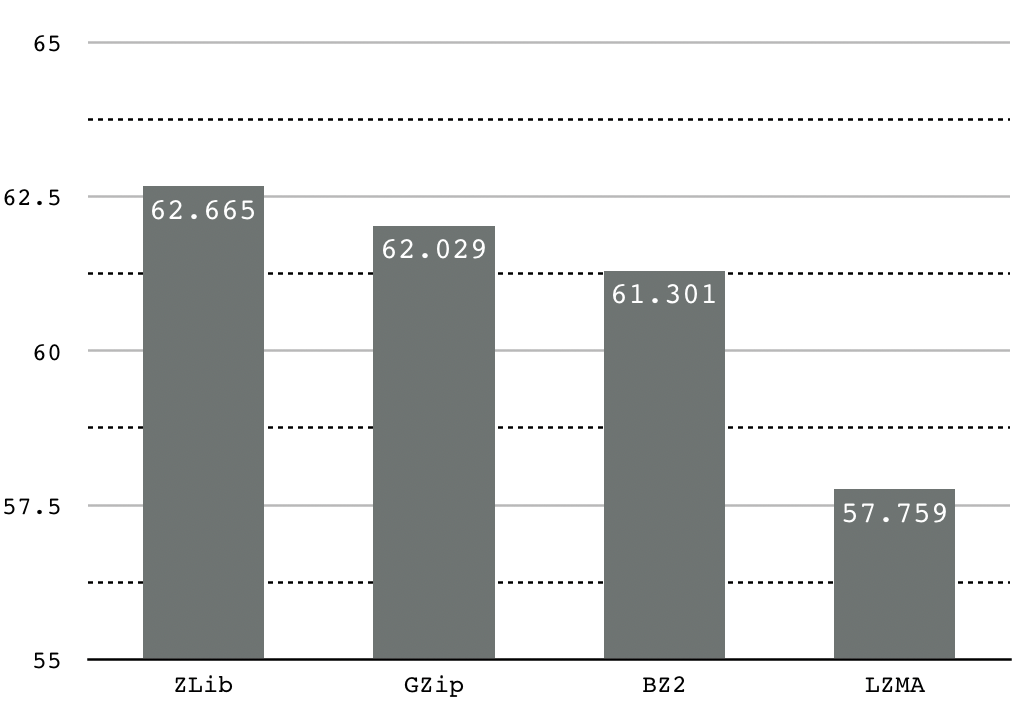
\includegraphics[width=0.5\textwidth]{sep-space.png}}
	\caption{نمودار فضای صرفه‌جویی}
	\label{fig:sep-space}
\end{figure}\\

نتایج آزمون بر اساس پارامتر سربار زمان ذیل چهار پیاده‌سازی مختلف در شکل
\ref{fig:sep-time}
 قابل‌مشاهده است.
\begin{figure}[ht]
	\centerline{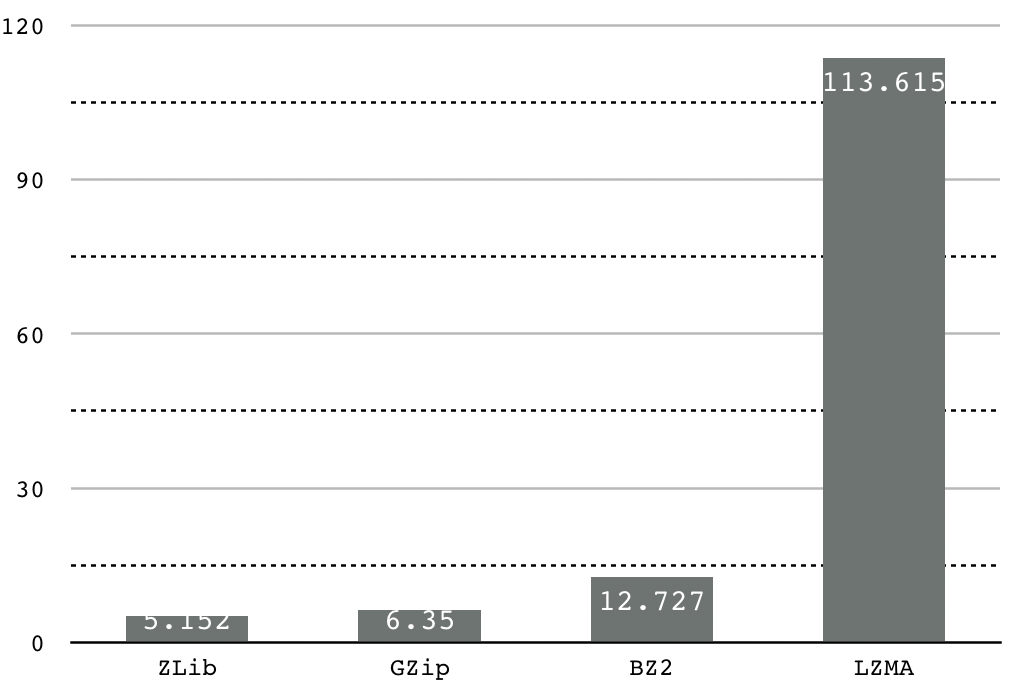
\includegraphics[width=0.5\textwidth]{sep-time.png}}
	\caption{نمودار سربار زمانی}
	\label{fig:sep-time}
\end{figure}\\

مقدار توان مصرفی به عنوان پارامتر مورد بحث ذیل چهار پیاده‌سازی مختلف در شکل
\ref{fig:sep-power}
 قابل‌مشاهده است.
\begin{figure}[ht]
	\centerline{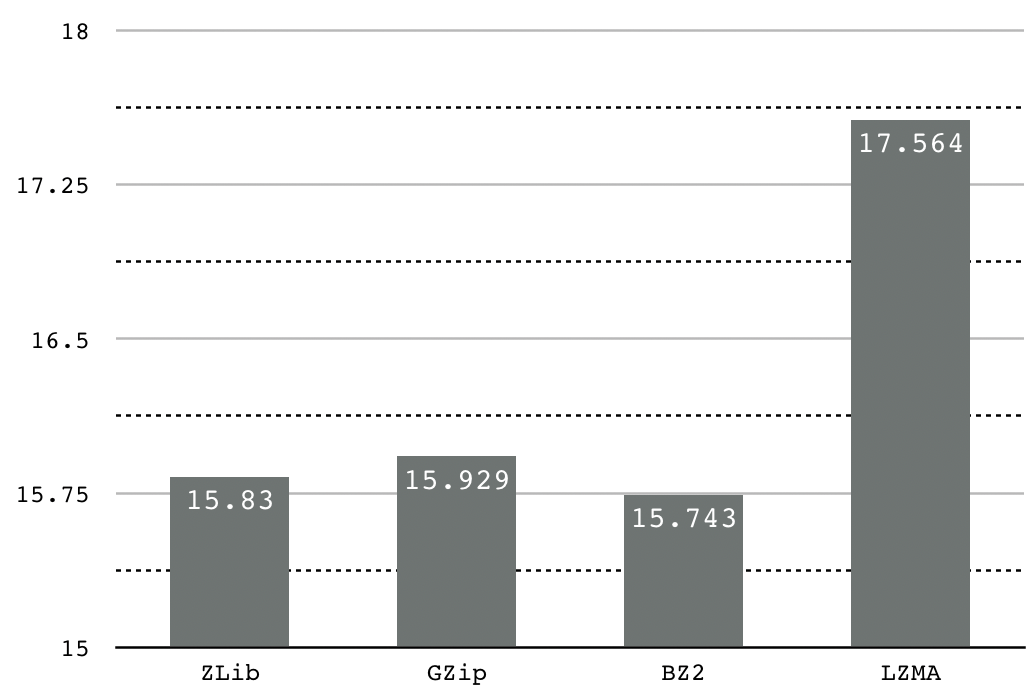
\includegraphics[width=0.5\textwidth]{sep-power.png}}
	\caption{نمودار توان مصرفی}
	\label{fig:sep-power}
\end{figure}\\

\subsection{فشرده‌سازی در حالت دسته‌ای}


نمودار فضای صرفه‌جویی‌شده برای چهار پیاده‌سازی انجام‌شده در
\ref{fig:chunk-space}
نشان داده شده‌است.
\begin{figure}[ht]
	\centerline{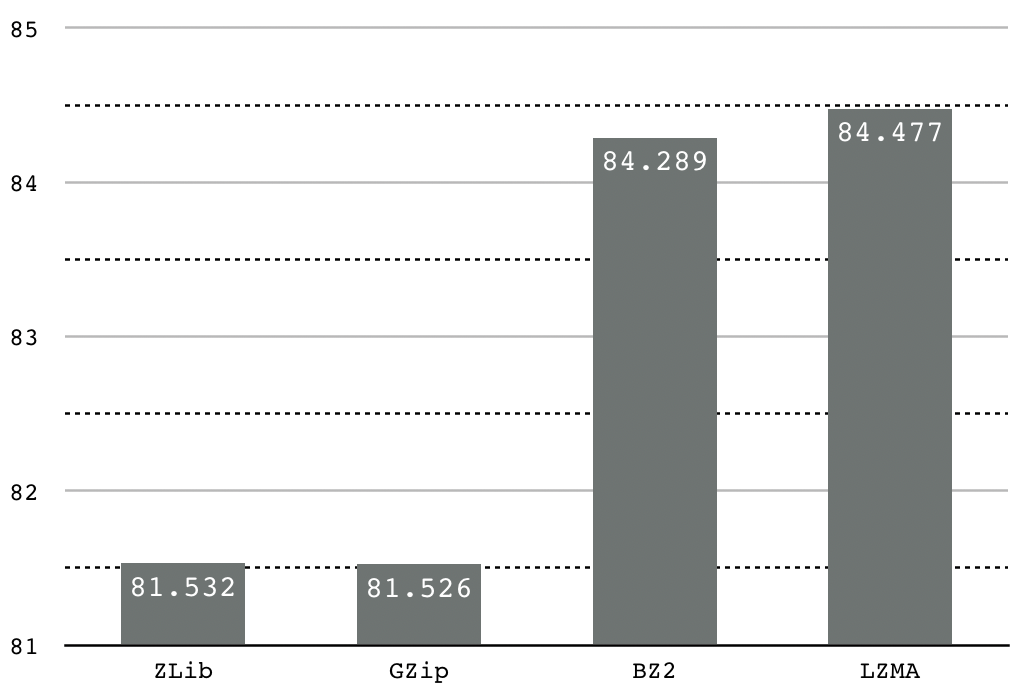
\includegraphics[width=0.5\textwidth]{chunk-space.png}}
	\caption{نمودار فضای صرفه‌جویی}
	\label{fig:chunk-space}
\end{figure}\\

نتایج به‌دست‌آمده برای پارامتر سربار زمان ذیل چهار پیاده‌سازی مختلف در شکل
\ref{fig:chunk-time}
دیده می‌شود.
\begin{figure}[ht]
	\centerline{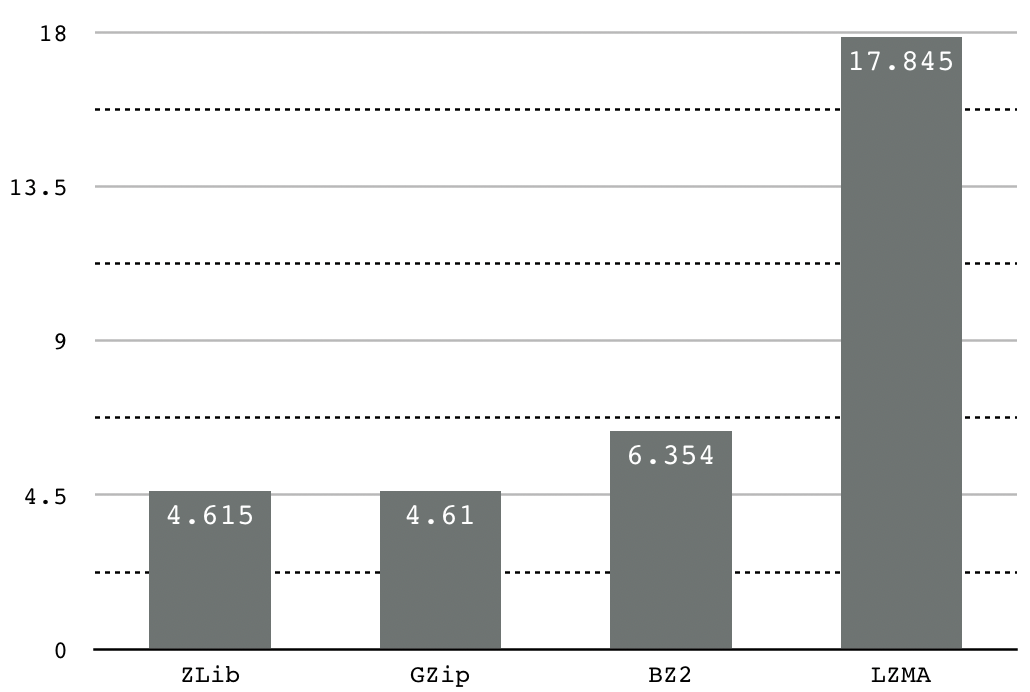
\includegraphics[width=0.5\textwidth]{chunk-time.png}}
	\caption{نمودار سربار زمانی}
	\label{fig:chunk-time}
\end{figure}\\

با درنظرگرفتن توان مصرفی به عنوان پارامتر مورد بحث در چهار پیاده‌سازی درنظرگرفته‌شده در شکل
\ref{fig:chunk-power}
قابل‌مشاهده است.
\begin{figure}[ht]
	\centerline{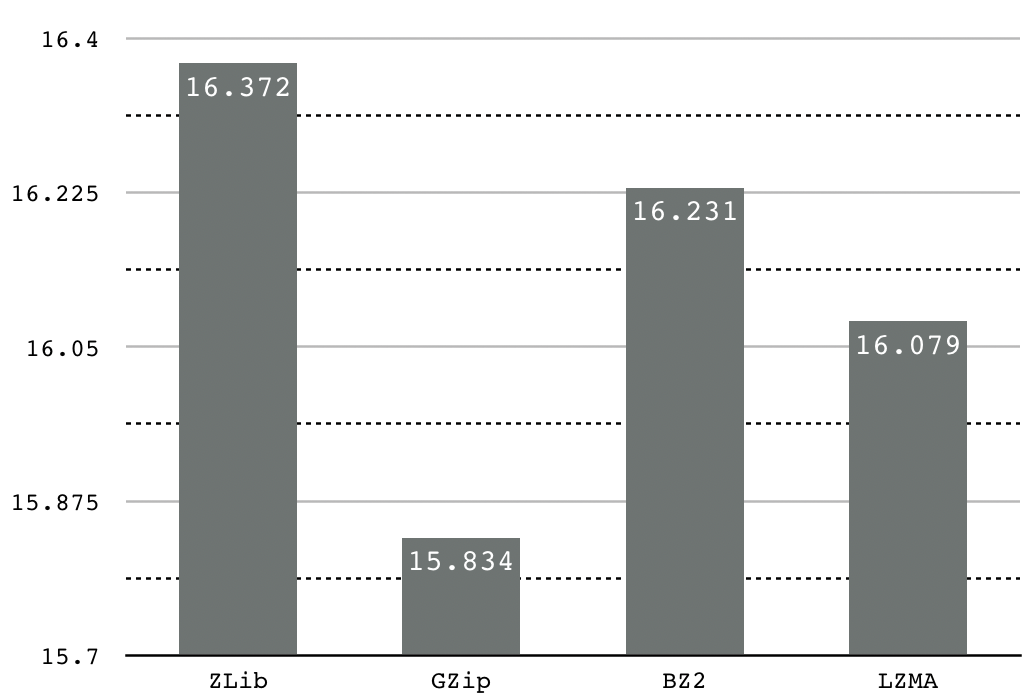
\includegraphics[width=0.5\textwidth]{chunk-power.png}}
	\caption{ نمودار توان مصرفی در حالت فشرده‌سازی دسته‌ای}
	\label{fig:chunk-power}
\end{figure}\\



\section{تحلیل نتایج}

پیاده‌سازی در دو حالت منفرد و دسته‌ای انجام و ذیل هرکدام از این آزمایش‌ها الگوریتم‌های مختلف فشرده‌سازی به کار گرفته شد. برای هرکدام از روش‌های استفاده‌شده، پارامترهای میزان فضای صرفه‌جویی‌شده،‌سربار زمانی و توان مصرفی ارزیابی شده‌است. با توجه به نتایج به‌دست‌آمده و نمودارهای متناظر می‌توان بین فشرده‌سازی‌های مختلف مقایسه انجام داد. 

با توجه به نتایج به‌دست‌آمده، همان‌طور که قبل از اجرای آزمون‌های متعدد با روش‌های فشرده‌سازی متفاوت پیش‌بینی می‌شد، حالت فشرده‌سازی دسته‌ای به مراتب میزان فضای صرفه‌جویی‌شده‌ی بیشتری را در اختیار ما قرار می‌داد. دلیل این امر آن است که آنتروپی با افزایش احتمال رخ‌دادن یک پیشامد کاهش می‌یابد و ذیل فشرده‌سازی دسته‌ای مقدار آنتروپی به حد چشم‌گیری کاهش می‌یابد. تأثیر این کاهش به حدی ا‌ست که بهترین حالت فشرده‌سازی دسته‌ای در مقایسه با بهترین حالت فشرده‌سازی منفرد بیشتر از ۲۰٪ بهبود را نشان می‌دهد.

از میان آزمایش‌های انجام‌شده بهترین الگوریتم فشرده‌سازی در هر دوحالت منفرد و دسته‌ای از منظر میزان فضای صرفه‌جویی‌شده به ترتیب ZLib و LZMA هستند. نکته‌ی حائز اهمیت در این‌جا آن است که الگوریتم LZMA در حالت فشرده‌سازی منفرد بدترین عملکرد را در میان الگوریتم‌های فشرده‌سازی بررسی‌شده دارد. این در حالی است که الگوریتم ZLib در حالت دسته‌ای نیز عملکرد قابل‌قبولی از خود به نمایش می‌گذارد. 

با بررسی توان مصرفی هرکدام از الگوریتم‌های فشرده‌سازی منتخب،‌ نتیجه می‌شود در حالت دسته‌ای الگوریتم ZLib بیشترین توان مصرفی و الگوریتم GZip کمترین توان مصرفی را موجب می‌شود. نکته‌ی شایان ذکر در این‌جا آن است که تفاوت میزان توان مصرفی این دو الگوریتم تفاوت معنادار و علمی با یکدیگر ندارد و می‌توان با تقریب خوبی این دو الگوریتم را از حیث میزان توان مصرفی برابر در نظر گرفت. درست است که توان مصرفی GZip از بین الگوریتم‌های بررسی‌شده کمترین مقدار را به خود اختصاص داده‌است اما از آن‌جایی که میزان فضای صرفه‌جویی‌شده توسط الگوریتم LZMA در حالت دسته‌ای بیشتر است و هم‌چنین توان مصرفی آن تفاوت قابل‌توجهی با GZip ندارد، می‌توان نتیجه گرفت که LZMA با در کنار هم قرار دادن توان مصرفی و میزان فضای صرفه‌جویی‌شده عملکرد بهتری دارد.

هم‌چنین در حالت فشرده‌سازی منفرد با توجه به نتایج به‌دست‌آمده مشاهده می‌شود که الگوریتم LZMA با اختلاف توان مصرفی بیشتری را در مقایسه با سایر الگوریتم‌های فشرده‌سازی صرف می‌کند. سایر الگوریتم‌های فشرده‌سازی  مورد آزمایش را می‌توان در یک مرتبه خواند. با در نظر گرفتن این موضوع، می‌توان استدلال نمود که الگوریتم فشرده‌سازی با میزان فضای صرفه‌جویی‌شده‌ی بیشتر، نسبت به سایر الگوریتم‌های فشرده‌سازی هم‌مرتبه از نظر توان مصرفی، اولویت دارد. در ادامه با توجه به برتری الگوریتم ZLib در مقایسه با الگوریتم LZMA از حیث میزان فضای صرفه‌جویی‌شده در حالت فشرده‌سازی منفرد و توان مصرفی کمتر الگوریتم ZLib می‌توان نتیجه گرفت که الگوریتم ZLib در حالت فشرده‌سازی منفرد برتری دارد.

\section{جمع‌بندی}

		% فصل چهارم: نتایج
% !TeX root=../main.tex
\chapter{بحث و نتیجه‌گیری}
%\thispagestyle{empty} 
\section{مقدمه}
تاکنون شما در پایان‌نامه‌ای که مشغول نوشتن آن هستید، پاسخ چهار سؤال را داده‌اید:
\begin{itemize}
	\item
	چرا تحقیق را انجام دادید؟ (مقدمه)
	\item
	دیگران در این زمینه‌ چه کارهایی کرده‌اند و تمایز کار شما با آنها؟ (مرور ادبیات)
	\item
	چگونه تحقیق را انجام دادید؟ (روش‌ها)
	\item
	چه از تحقیق به دست آوردید؟ (یافته‌ها)
\end{itemize}
حال زمان آن فرا رسیده که با توجه به تمامی مطالب ذکر شده، در نهایت به سؤال آخر پاسخ دهید:
\begin{itemize}
	\item
	چه برداشتی از یافته‌های تحقیق کردید؟ (نتیجه‌گیری)
\end{itemize}
در واقع در این بخش، هدف، پاسخ به این سوال است که چه برداشتی از یافته‌ها کردید و این یافته‌ها چه فایده‌ای دارند؟

نتیجه‌گیری مختصری بنویسید. ارائهٔ داده‌ها، نتایج و یافته‌ها در فصل چهارم ارائه می‌شود. در این فصل تفاوت، تضاد یا تطابق بین نتایج تحقیق با نتایج دیگر محققان باید ذکر شود.
\emph{تفسیر و تحلیل نتایج نباید بر اساس حدس و گمان باشد}،
بلکه باید
\textbf{برمبنای نتایج عملی استخراج‌شده}
از تحقیق و یا
\textbf{استناد به تحقیقات دیگران}
باشد.
با توجه به حجم و ماهیت تحقیق و با صلاحدید استاد راهنما، این فصل می‌تواند تحت عنوانی دیگر بیاید یا به دو فصل جداگانه با عناوین مناسب، تفکیک شود. این فصل فقط باید به جمع‌بندی دست‌آوردهای فصل‌های سوم و چهارم محدود و از ذکر موارد جدید در آن خودداری شود. در عنوان این فصل، به جای کلمهٔ «تفسیر» می‌توان از واژگان «بحث» و «تحلیل» هم استفاده کرد. این فصل شاید مهم‌ترین فصل پایان‌نامه باشد.

در این فصل خلاصه‌ای از یافته‌های تحقیق جاری ارائه می‌شود. این فصل می‌تواند حاوی یک مقدمه، شامل مروری اجمالی بر مراحل انجام تحقیق باشد (حدود یک صفحه). مطالب پاراگراف‌بندی شود و هر پاراگراف به یک موضوع مستقل اختصاص یابد. فقط به ارائهٔ یافته‌ها و دست‌آوردها بسنده شود و
\emph{از تعمیم بی‌مورد نتایج خودداری شود.}
تا حد امکان از ارائهٔ 
\emph{جداول و نمودارها در این فصل اجتناب شود.}
از ارائهٔ 
\emph{عناوین کلی}
در حوزهٔ تحقیق و قسمت پیشنهاد تحقیقات آتی خودداری شود و کاملاً در چارچوب و زمینهٔ مربوط به تحقیق جاری باشد. این فصل حدود ۱۰-۱۵ صفحه است.

\section{محتوا}
به ترتیب شامل موارد زیر است:

\subsection{جمع‌بندی}
خلاصه‌ای از تمام یافته‌ها و دست‌آوردهای تحقیق جاری است.

\subsection{نوآوری}
این قسمت، نوآوری تحقیق را بر اساس یافته‌های آن تشریح می‌کند. که دارای دو بخش اصلی است:
\begin{enumerate}
	\item
	نوآوری تئوری، یعنی تمایز تئوریک کار با کارهای محققین قبلی.
	\item
	نوآوری عملی، یعنی توصیه‌های محقق به صنعت برای بهبود بخشیدن به کارها، بر اساس یافته‌های تحقیق.
\end{enumerate}

\subsection{پیشنهادها}
این بخش، عناوین و موضوعات پیشنهادی را برای تحقیقات آتی،
\emph{بیشتر در زمینهٔ مورد بحث در آینده}
ارائه می‌کند.

\subsection{محدودیت‌ها}
در اینجا انواع محدودیت‌های تحقیق تشریح می‌شوند؛ از جمله، محدودیت‌هایی که کنترل آن از عهده محقق خارج است، مانند انتخاب نوع یافته‌ها؛ و همچنین دیگر محدودیت‌هایی که کنترل آن در دست محقق است، مانند موضوع و محل تحقیق و ... . تأثیر این محدودیت‌ها بر یافته‌های تحقیق در این قسمت شرح داده می‌شوند.		% فصل پنجم: بحث و نتیجه‌گیری

% مراجع
% اگر از استیل‌های natbib استفاده می‌کنید باید دو خط را در فایل commands.tex تغییر دهید.
\pagestyle{empty}
{
\small
\onehalfspacing
\bibliographystyle{plain-fa} % or plainnat-fa for author-date
\bibliography{./tex/MyReferences}
}

\pagestyle{fancy}

% \appendix
% فصلهای پس از این قسمت به عنوان ضمیمه خواهند آمد.

% دستورات لازم برای تبدیل «فصل آ» به «پیوست آ» در فهرست مطالب
\addtocontents{toc}{
    \protect\renewcommand\protect\cftchappresnum{\appendixname~}%
    \protect\setlength{\cftchapnumwidth}{\mylenapp}}
    
\let\Chapter\chapter
% دستورات لازم برای شماره‌گذاری صفحات پیوست‌ها بشکل آ-۱ (فعلا با glossaries سازگار نیست)
%\pretocmd{\chapter}{
%  \clearpage
%  \pagenumbering{arabic}
%  \renewcommand*{\thepage}{\rl{\thechapter-\arabic{page}}}}{}{}
%%%%%%%%%%%%%%%%%%%%%%%%%%%%%%%%%%%%%
    

%% !TeX root=../main.tex

\chapter{آشنایی سریع با برخی دستورات لاتک}
\label{app:latexIntro}
%\thispagestyle{empty}
در این فصل ویژگی‌های مهم و پرکاربرد زی‌پرشین و لاتک معرفی می‌شود. برای راهنمایی بیشتر و به‌کاربردن ویژگی‌های پیشرفته‌تر به راهنمای زی‌پرشین و راهنمای لاتک مراجعه کنید. برای آگاهی از دستورات لاتک که این خروجی را تولید کرده‌اند فایل \lr{appendix1.tex} را ملاحظه فرمایید.
\footnote{بیشتر مطالب این بخش از مثال 
\lr{xepersian\_example.tex}
گرفته شده‌اند که توسط آقای امیرمسعود پورموسی آماده شده است.}

\section{بندها و زیرنویس‌ها}
هر جایی از نوشتهٔ خود، اگر می‌خواهید به سر سطر بروید و یک بند (پاراگراف) تازه را آغاز کنید، باید یک خط را خالی بگذارید%
\footnote{یعنی دوبار باید کلید \lr{Enter} را بزنید.}
 مانند این:

حالا که یک بند تازه آغاز شده است، یک زیرنویس انگلیسی%
\LTRfootnote{English Footnote!}
 هم می‌نویسیم!
\section{فرمول‌های ریاضی}
\label{formula}

اینجا هم یک فرمول می‌آوریم که شماره دارد:
\begin{equation}\label{eq:yek}
A=\frac{c}{d}+\frac{q^2}{\sin(\omega t)+\Omega_{12}}
\end{equation}
در لاتک می‌توان به کمک فرمان 
\lr{\textbackslash label\{\}}
به هر فرمول یک نام نسبت داد. در فرمول بالا نام \lr{eq:yek} را برایش گذاشته‌ایم (پروندهٔ \lr{tex} همراه با این مثال را ببینید). این نام ما را قادر می‌کند که بعداً بتوانیم با فرمان
\lr{\textbackslash ref\{eq:yek\}}
به آن فرمول با شماره ارجاع دهیم. یعنی بنویسیم فرمول \ref{eq:yek}. 
لاتک خودش شمارهٔ این فرمول‌ها را مدیریت می‌کند.\footnote{یعنی اگر بعداً فرمولی قبل از این فرمول بنویسیم، خودبه‌خود شمارهٔ این فرمول و شمارهٔ ارجاع‌ها به این فرمول یکی زیاد می‌شود. دیگر نگران شماره‌گذاری فرمول‌های خود نباشید!} این هم یک فرمول که شماره ندارد:
$$A=|\vec{a}\times \vec{b}| + \sum_{n=0}^\infty C_{ij}$$

این هم عبارتی ریاضی مانند 
$\sqrt{a^2+b^2}$
 که بین متن می‌آید.
\subsection{یک زیربخش}
\label{zirbakhsh}

این زیربخش \ref{zirbakhsh} است؛ یعنی یک بخش درون بخش \ref{formula} است.
\subsubsection{یک زیرزیربخش}
این هم یک زیرزیربخش است. در لاتک می‌توانید بخش‌های تودرتو در نوشته‌تان تعریف کنید تا ساختار منطقی نوشته را به خوبی نشان دهید. می‌توانید به این بخش‌ها هم با شماره ارجاع دهید، مثلاً بخش فرمول‌های ریاضی شماره‌اش \ref{formula} است.
\section{نوشته‌های فارسی و انگلیسی مخلوط}
نوشتن یک کلمهٔ انگلیسی بین متن فارسی بدیهی است، مانند Example در این جمله.\footnote{هرچند بهتر است باز هم آن کلمه را مانند \lr{Example} در این جمله بنویسید.}
نوشتن یک عبارت چندکلمه‌ای مانند
 \lr{More than one word} کمی پیچیده‌تر است.

اگر ناگهان تصمیم بگیرید که یک بند کاملاً انگلیسی را بنویسید، باید:
\begin{latin}
This is an English paragraph from left to right. You can write as much as you want in it.
\end{latin}
\section{افزودن تصویر به نوشته}
پروندهٔ تصویر دلخواه خود را در کنار پروندهٔ \lr{tex} قرار دهید. سپس به روش زیر تصویر را در نوشتهٔ خود بیاورید:
\begin{latin}
\begin{verbatim}
\includegraphics{YourImageFileName}
\end{verbatim}
\end{latin}
به تصویرها هم مانند فرمول‌ها و بخش‌ها می‌توان با شماره ارجاع داد. مثلاً تصویر \ref{fig:shir} یک شیر علاقه‌مند به لاتک را در حال دویدن نشان می‌دهد. برای جزئیات بیشتر دربارهٔ روش گذاشتن تصویرها در نوشته باید راهنماهای لاتک را بخوانید.
\begin{figure}[ht]
\centerline{
\includegraphics[width=5cm]{lion}}
\caption{در این تصویر یک شیر علاقه‌مند به لاتک را در حال دویدن می‌بینید.}
\label{fig:shir}
\end{figure}

به تصویرها هم مانند فرمول‌ها و بخش‌ها می‌توان با شماره ارجاع داد. مثلاً تصویر بالا شماره‌اش \ref{fig:shir} است. برای جزئیات بیشتر دربارهٔ روش گذاشتن تصویرها در نوشته باید راهنماهای لاتک را بخوانید.

\section{محیط‌های شمارش و نکات}
برای فهرست‌کردن چندمورد، اگر ترتیب برایمان مهم نباشد:
\begin{itemize}
\item مورد یکم
\item مورد دوم
\item مورد سوم
\end{itemize}
و اگر ترتیب برایمان مهم باشد:
\begin{enumerate}
\item مورد یکم
\item مورد دوم
\item مورد سوم
\end{enumerate}
می‌توان موردهای تودرتو داشت:
\begin{enumerate}
\item مورد ۱
\item مورد ۲
\begin{enumerate}
\item مورد ۱ از ۲
\item مورد ۲ از ۲
\item مورد ۳ از ۲
\end{enumerate}
\item مورد ۳
\end{enumerate}
شماره‌گذاری این موردها را هم لاتک انجام می‌دهد.

\section{تعریف و قضیه}
برای ذکر تعریف، قضیه و مثال مثالهای ذیل را ببینید.
\begin{definition}
مجموعه همه ارزیابی‌های  (پیوسته)  روی $(X,\tau)$، دامنه توانی احتمالی
\index{دامنه توانی احتمالی}
$ X $
نامیده می‌شود.
\end{definition}
\begin{theorem}[باناخ-آلااغلو]
\index{قضیه باناخ-آلااغلو}
اگر $ V $ یک همسایگی $ 0 $ در فضای برداری 
\index{فضای!برداری}
 توپولوژیکی $ X $ باشد و 
\begin{equation}\label{eq1}
K=\left\lbrace \Lambda \in X^{*}:|\Lambda x|\leqslant 1 ; \ \forall x\in V\right\rbrace,
\end{equation}
آنگاه $ K $،  ضعیف*-فشرده است که در آن، $ X^{*} $ دوگان
\index{فضای!دوگان}
 فضای برداری توپولوژیکی $ X $ است به ‌طوری که عناصر آن،  تابعی‌های 
خطی پیوسته
\index{تابعی خطی پیوسته}
 روی $X$ هستند.
\end{theorem}
تساوی \eqref{eq1} یکی از مهم‌ترین تساوی‌ها در آنالیز تابعی است که در ادامه، به وفور از آن استفاده می‌شود.
\begin{example}
برای هر فضای مرتب، گردایه 
$$U:=\left\lbrace U\in O: U=\uparrow U\right\rbrace $$
از مجموعه‌های بالایی باز، یک توپولوژی تعریف می‌کند که از توپولوژی اصلی، درشت‌تر  است.
\end{example}
حال تساوی 
\begin{equation}\label{eq2}
\sum_{n=1}^{+\infty} 3^{n}x+7x=\int_{1}^{n}8nx+\exp{(2nx)}
\end{equation}
را در نظر بگیرید. با مقایسه تساوی \eqref{eq2} با تساوی \eqref{eq1} می‌توان نتیجه گرفت که ...


\section{چگونگی نوشتن و ارجاع به مراجع}
\label{Sec:Ref}


در لاتک به راحتی می‌توان مراجع خود را نوشت و به آنها ارجاع داد. به عنوان مثال برای معرفی کتاب گنزالس \cite{Gonzalez02book} به عنوان یک مرجع می‌توان آنرا به صورت زیر معرفی نمود:

\singlespacing
\begin{LTR}
\begin{verbatim}
\bibitem{Gonzalez02book}
Gonzalez, R.C., and Woods, R.E. {\em Digital Image Processing}, 3rd ed..
Prentice-Hall, Inc., Upper Saddle River, NJ, USA, 2006.
\end{verbatim}
\end{LTR}
\doublespacing

در دستورات فوق \lr{Gonzalez02book}  برچسبی است که به این مرجع داده شده است و با استفاده از دستور 
\verb!\cite{Gonzalez02book}!
می‌توان به آن ارجاع داد؛ بدون این که شماره‌اش را در فهرست مراجع‌مان بدانیم.

اگر این اولین مرجع ما باشد در قسمت مراجع به صورت زیر خواهد آمد:\\
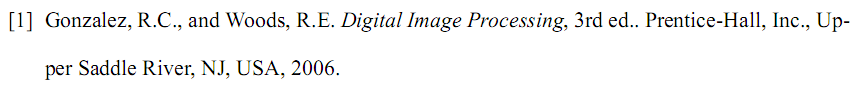
\includegraphics[width=\textwidth]{gonzalez.png}

این شیوهٔ تعریف مراجع بسیار ابتدایی است و اگر فرمت مراجع، ترتیب یا تعداد آنها را خواسته باشید تغییر دهید، به عنوان مثال ابتدا حرف اول نام نویسنده بیاید و سپس نام خانوادگی، باید همه کارها را به صورت دستی انجام دهید!
چون در یک \پ یا مقاله باید کنترل کاملی بر مراجع خود داشته باشید و به راحتی بتوانید قالب مراجع را عوض کنید، بنابراین می‌بایست از \lr{Bib\TeX} استفاده کنید که درپیوست  \ref{app:refMan} به  آن پرداخته خواهد شد.
		% پیوست اول: آشنایی مقدماتی با لاتک
%% !TeX root=../main.tex

\chapter{‌جدول، نمودار و الگوریتم در لاتک}
\label{app:latex:more}
%\thispagestyle{empty}

در این بخش نمونه مثالهایی از جدول، شکل، نمودار، الگوریتم و معادلات ریاضی را در لاتک خواهیم دید.
دقت کنید که در پایان‌نامه‌ها و مقالات، باید قاعدهٔ «ارجاع به جلو%
\LTRfootnote{Forward Referencing}»
رعایت شود؛ یعنی ابتدا در متن به شمارهٔ شکل، جدول یا معادله اشاره شود و بعد از آن (زیر آن) خود شکل، جدول یا معادله رسم شود. (توضیحات بیشتر در قسمت
\ref{sec:floatObjs}).

\section{جدول}
دستور اصلی برای رسم جدول در لاتک 
\verb|tabular|
می‌باشد که جدول
\eqref{tab:motionModels}
با استفاده از آن کشیده شده است؛ در
\verb|tabular|
عرض جدول برابر با مجموع عرض ستون‌ها و حداکثر مساوی عرض متن است.
\begin{table}[ht]
\caption{مدلهای تبدیل.}
\label{tab:motionModels}
\centering
\onehalfspacing
\begin{tabular}{|r|c|l|r|}
	\hline نام مدل & درجه آزادی & تبدیل مختصات & توضیح \\ 
	\hline انتقالی & ۲ & $\begin{aligned} x'=x+t_x \\ y'=y+t_y \end{aligned}$  &  انتقال دوبعدی\\ 
	\hline اقلیدسی & ۳ & $\begin{aligned} x'=x\cos\theta - y\sin\theta+t_x \\ y'=x\sin\theta+y\cos\theta+t_y \end{aligned}$  &  انتقالی+دوران \\ 
	\hline 
\end{tabular} 
\end{table}

برای اینکه عرض جدول قابل کنترل باشد، باید از دستورات
\verb|tabularx|،
\verb|tabulary| یا
\verb|tabu|
استفاده کرد که راهنمای آنها در اینترنت وجود دارد.
مثلاً جدول
\ref{tab:motionModelsCont}
با
\verb|tabularx|
رسم شده که عرض جدول در آن ثابت بوده و ستون‌های از نوع
\verb|X|
عرض خالی جدول را پر می‌کنند.
\begin{table}[ht]
	\caption{مدلهای تبدیل دیگر.}
	\label{tab:motionModelsCont}
	\centering
	\onehalfspacing
	\begin{tabularx}{\textwidth}{|r|c|l|X|}
		\hline نام مدل & درجه آزادی & تبدیل مختصات & توضیح \\ 
		\hline مشابهت & ۴ & $\begin{aligned} x'=sx\cos\theta - sy\sin\theta+t_x \\ y'=sx\sin\theta+sy\cos\theta+t_y  \end{aligned}$  & اقلیدسی+تغییرمقیاس \\ 		
		\hline آفین & ۶ & $\begin{aligned} x'=a_{11}x+a_{12}y+t_x \\ y'=a_{21}x+a_{22}y+t_y \end{aligned}$  & مشابهت+اریب‌شدگی \\
		\hline
	\end{tabularx}
\end{table}

\section{معادلات ریاضی و ماتریس‌ها}
تقریباً هر آنچه دانشجویان برای نوشتن فرمول‌های ریاضی لازم دارند، در کتاب 
\lr{mathmode}
آمده است. کافیست در خط فرمان، دستور زیر را وارد کنید:
\begin{latin}
	\texttt{texdoc mathmode}
\end{latin}
متن زیر شامل انواعی از اشیاء ریاضی است که با ملاحظه کدش می‌توانید با دستورات آن آشنا شوید.\\
شناخته‌شده‌ترین روش تخمین ماتریس هوموگرافی الگوریتم تبدیل خطی مستقیم (\lr{DLT\LTRfootnote{Direct Linear Transform}}) است.  فرض کنید چهار زوج نقطهٔ متناظر در دو تصویر در دست هستند،  $\mathbf{x}_i\leftrightarrow\mathbf{x}'_i$   و تبدیل با رابطهٔ
  $\mathbf{x}'_i = H\mathbf{x}_i$
  نشان داده می‌شود که در آن:
\[\mathbf{x}'_i=(x'_i,y'_i,w'_i)^\top  \]
و
\[ H=\left[
\begin{array}{ccc}
h_1 & h_2 & h_3 \\ 
h_4 & h_5 & h_6 \\ 
h_7 & h_8 & h_9
\end{array} 
\right]\]
رابطه زیر را برای الگوریتم  \eqref{alg:DLT} لازم داریم.
\begin{equation}
\label{eq:DLT_Ah}
\left[
\begin{array}{ccc}
	0^\top & -w'_i\mathbf{x}_i^\top & y'_i\mathbf{x}_i^\top \\ 
	w'_i\mathbf{x}_i & 0^\top & -x'_i\mathbf{x}_i^\top \\ 
	- y'_i\mathbf{x}_i^\top & x'_i\mathbf{x}_i^\top & 0^\top
\end{array} 
\right]
\left(
\begin{array}{c}
	\mathbf{h}^1 \\ 
	\mathbf{h}^2 \\ 
	\mathbf{h}^3
\end{array} 
\right)=0
\end{equation}

\section{الگوریتم با دستورات فارسی}
با مفروضات فوق، الگوریتم \lr{DLT} به صورت نشان داده شده در الگوریتم \eqref{alg:DLT}  خواهد بود.
\begin{algorithm}[ht]
\onehalfspacing
\caption{الگوریتم \lr{DLT} برای تخمین ماتریس هوموگرافی.} \label{alg:DLT}
\begin{algorithmic}[1]
\REQUIRE $n\geq4$ زوج نقطهٔ متناظر در دو تصویر 
${\mathbf{x}_i\leftrightarrow\mathbf{x}'_i}$،\\
\ENSURE ماتریس هوموگرافی $H$ به نحوی‌که: 
$\mathbf{x}'_i = H \mathbf{x}_i$.
  \STATE برای هر زوج نقطهٔ متناظر
$\mathbf{x}_i\leftrightarrow\mathbf{x}'_i$ 
ماتریس $\mathbf{A}_i$ را با استفاده از رابطهٔ \ref{eq:DLT_Ah} محاسبه کنید.
  \STATE ماتریس‌های ۹ ستونی  $\mathbf{A}_i$ را در قالب یک ماتریس $\mathbf{A}$ ۹ ستونی ترکیب کنید. 
  \STATE تجزیهٔ مقادیر منفرد \lr{(SVD)}  ماتریس $\mathbf{A}$ را بدست آورید. بردار واحد متناظر با کمترین مقدار منفرد جواب $\mathbf{h}$ خواهد بود.
  \STATE  ماتریس هوموگرافی $H$ با تغییر شکل $\mathbf{h}$ حاصل خواهد شد.
\end{algorithmic}
\end{algorithm}

\section{الگوریتم با دستورات لاتین}
الگوریتم \ref{alg:RANSAC} یک الگوریتم با دستورات لاتین است.

\begin{algorithm}[ht]
\onehalfspacing
\caption{الگوریتم \lr{RANSAC} برای تخمین ماتریس هوموگرافی.} \label{alg:RANSAC}
\begin{latin}
\begin{algorithmic}[1]
\REQUIRE $n\geq4$ putative correspondences, number of estimations, $N$, distance threshold $T_{dist}$.\\
\ENSURE Set of inliers and Homography matrix $H$.
\FOR{$k = 1$ to $N$}
  \STATE Randomly choose 4 correspondence,
  \STATE Check whether these points are colinear, if so, redo the above step
  \STATE Compute the homography $H_{curr}$ by DLT algorithm from the 4 points pairs,
  \STATE $\ldots$ % الگوریتم کامل نیست
  \ENDFOR
  \STATE Refinement: re-estimate H from all the inliers using the DLT algorithm.
\end{algorithmic}
\end{latin}
\end{algorithm}

\section{درج کد}
درج کد به زبان‌های مختلف به سادگی امکان‌پذیر است. برنامه
\ref{code:matlabEx}
یک قطعه کد
\lr{MATLAB}
را نشان می‌دهد.
\singlespacing
\begin{figure}
	\begin{LTR}
		\lstinputlisting[language=MATLAB, caption={نمونه کد \lr{MATLAB}}, label={code:matlabEx}]{MatlabExample.m}
	\end{LTR}
\end{figure}
\doublespacing

\section{تصویر}
نمونهٔ یک تصویر را در فصل قبل دیدیم. دو تصویر شیر کنار هم را نیز در شکل
\ref{fig:twoLion}
مشاهده می‌کنید.
\begin{figure}[ht]
\centering 
\subfloat[شیر ۱]{ \label{fig:twolion:one}

\includegraphics[width=0.3\textwidth]{lion}}
%\hspace{2mm}
\subfloat[شیر ۲]{ \label{fig:twolion:two}

\includegraphics[width=0.3\textwidth]{lion}}%
\caption{دو شیر}
\label{fig:twoLion} %% label for entire figure
\end{figure}

\section{نمودار}
لاتک بسته‌هایی با قابلیت‌های زیاد برای رسم انواع مختلف نمودارها دارد. مانند بسته‌های \lr{Tikz} و  \lr{PSTricks}. توضیح اینها فراتر از این پیوست کوچک است.%
\footnote{
مثال‌هایی از بکارگیری بسته
\lr{Tikz}
را می‌توانید در
\url{http://www.texample.net/tikz/examples/}
ببینید. توصیه می‌شود دانشجویانی که قصد درج اشکالی مانند گراف را در سند خود دارند، مثالهایی از سایت مذکور را ملاحظه فرمایند.
}
یک نمودار رسم شده با بسته‌ی 
\lr{TikZ}
 در شکل 
\ref{fig:parabola}
نشان داده شده است.
\begin{figure}[t]
\centering
\begin{tikzpicture}[scale=2.5]
  \shade[top color=blue,bottom color=gray!50] 
      (0,0) parabola (1.5,2.25) |- (0,0);
  \draw (1.05cm,2pt) node[above] 
      {$\displaystyle\int_0^{3/2} \!\!x^2\mathrm{d}x$};

  \draw[style=help lines] (0,0) grid (3.9,3.9)
       [step=0.25cm]      (1,2) grid +(1,1);

  \draw[->] (-0.2,0) -- (4,0) node[right] {$x$};
  \draw[->] (0,-0.2) -- (0,4) node[above] {$f(x)$};

  \foreach \x/\xtext in {1/1, 1.5/1\frac{1}{2}, 2/2, 3/3}
    \draw[shift={(\x,0)}] (0pt,2pt) -- (0pt,-2pt) node[below] {$\xtext$};

  \foreach \y/\ytext in {1/1, 2/2, 2.25/2\frac{1}{4}, 3/3}
    \draw[shift={(0,\y)}] (2pt,0pt) -- (-2pt,0pt) node[left] {$\ytext$};

  \draw (-.5,.25) parabola bend (0,0) (2,4) node[below right] {$x^2$};
\end{tikzpicture}
\caption{یک نمودار زیبا با ارقام فارسی و قابلیت بزرگ‌نمایی بسیار، بدون از دست دادن کیفیت.}
\label{fig:parabola}
\end{figure}

\section{نحوه قرارگیری اشیای شناور}
\label{sec:floatObjs}
شکل‌ها، جداول و الگوریتم‌ها در لاتک اشیای شناور محسوب می‌شوند؛ یعنی خود لاتک تصمیم می‌گیرد آنها را در کجای صفحه ترسیم کند تا زیباتر باشد. اما می‌توان به لاتک توصیه کرد که آن را در قسمت خاصی از صفحه رسم کند. برای اینکه قاعدهٔ «ارجاع به جلو» رعایت شود باید فقط از پرچم
\verb|[ht]|
استفاده کرد، که می‌گوید اگر جا شد شکل را دقیقاً در همین مکان و در غیراینصورت در بالای صفحه بعد رسم کن.
بنابراین دستورات درج تصویر، جدول و الگوریتم به صورت زیر باید باشند:

\begin{latin}
\begin{verbatim}
	\begin{figure/table/algorithm}[ht]
		...
	\end{figure/table/algorithm}
\end{verbatim}
\end{latin}		% پیوست دوم: جدول، نمودار و الگوریتم در لاتک
%% !TeX root=../main.tex
\chapter{مراجع، واژه‌نامه و حاشیه‌نویسی}
\label{app:refMan}
%\thispagestyle{empty}

\section{مراجع و نقل‌قول‌ها}
\label{sec:refUsage}
منابعِ پایان‌نامه، پایه و اساس تحقیق شما به حساب می‌آیند و ضرورت انجام مطالعه و روش‌های به کار رفته در بسیاری از قسمت‌های آن، به کمک منابع صورت می‌گیرد. در استفاده از مراجع علمی در پایان‌نامه، باید سعی کنید بیشتر از
\textbf{منابع چاپ‌شده و مهم}
استفاده کنید و
\emph{ارجاع به داده‌های چاپ نشده، خلاصه‌ها و پایان‌نامه‌ها، سبب به‌هم‌خوردگی و کاهش اعتبار قسمت ارجاع منابع می‌شود.}
استفاده از منابع و نقل قول‌هایی به تحقیق شما ارزش می‌دهند که
\textbf{در راستای هدف تحقیق بوده و به آن اعتبار ببخشند.}
برخی از دانش‌جویان تصوّر می‌کنند که کثرت نقل‌قول‌ها و ارجاعات زیاد، مهم‌ترین معیار علمی شدن پایان‌نامه است؛ حال آنکه استناد به تعداد کثیری از منابع بدون مطالعه دقیق آنها و استفادهٔ مستقیم در پایان‌نامه، می‌تواند نشان‌دهندهٔ عدم احساس امنیت نویسنده باشد!

دو روش برای استفاده از نتایج، جملات، داده‌ها و روش‌های دیگران وجود دارد. یکی نقل‌قول مستقیم و دقیق است و دیگری استفاده غیرمستقیم در متن مقاله، که در ادامه به قواعد این دو نوع نقل‌قول و ارجاع‌دهی اشاره می‌کنیم:
\begin{description}
	\item[نقل‌قول مستقیم:]
	نقل‌قول مستقیم باید دقیق و بدون هیچ تغییری در جملات باشد. بهتر است این‌گونه نقل‌قول‌ها تا حد امکان کوتاه باشد. جملات کوتاه داخل گیومه قرار می‌گیرند و باید به منبع دقیق آن، طبق روش ارجاع‌دهی به منابع، اشاره شود. به عنوان مثال در
	\cite{persianbib87userguide}
	آمده است که:
	\begin{quote}
		«با استفاده از فیلد
		\lr{AUTHORFA}
		می‌توان معادل فارسی نام نویسندگان مقالات لاتین را در متن داشت. معمولاً در اسناد فارسی خواسته می‌شود که پس از ذکر معادل فارسی نام نویسنده، نام لاتین نویسنده(ها) به عنوان پاورقی درج شود
		\citep{persianbib87userguide}.»
	\end{quote}
	\item[نقل‌قول غیرمستقیم:]
	نقل‌قول غیرمستقیم به معنی استفاده از ایده‌ها، نتایج، روش‌ها و داده‌های دیگران در درون متنِ پایان‌نامه، ولی به سبک خودتان و متناسب و هماهنگ با روند پایان‌نامهٔ شماست. در این حالت نیز باید متناسب با شیوهٔ ارجاع‌دهی به آن استناد شود.
\end{description}

با توجه به وجود سبک‌های مختلف ارجاع‌دهی، باید
\textbf{روش قابل قبول و یکسانی}
در طول پایان‌نامه برای اشاره به مراجع در متن و همچنین تهیه فهرست مراجع در انتهای پایان‌نامه بکار رود. مثلاً برای پایان‌نامه‌های مهندسی می‌توان از سبک ارجاع‌دهی
\lr{IEEE}%
\LTRfootnote{\url{http://www.ieee.org/documents/ieeecitationref.pdf}}
یا
\lr{acm}
استفاده کرد. طبیعتاً باید تناظر یک‌به‌یک بین فهرست مراجع در انتهای گزارش و مراجع مورد استفاده در متن باشد%
\footnote{البته گاهی ممکن است محقق مرجعی را مورد مطالعه قرار داده لیکن در متن به آن اشاره نکرده باشد؛ برخی معتقدند در این موارد نیز آوردن آن در فهرست مراجع، اشکالی ندارد، به این شرط که از عنوان «فهرست منابع» به جای «فهرست مراجع» استفاده شود.}.

برای سهولت مدیریت مراجعِ \پ%
، اکیداً توصیه می‌شود از یک ابزار «مدیریت منابع» (با خروجی
\texorpdfstring{\lr{Bib\TeX}}{Bib\TeX}%
) همچون
\lr{Mendeley}،
\lr{Zotero},
\lr{EndNote}
یا
\lr{Citavi}
استفاده کنید.

\subsection{ مدیریت مراجع با  \texorpdfstring{\lr{Bib\TeX}}{Bib\TeX}}
در بخش \ref{Sec:Ref} اشاره شد که با دستور 
 \lr{\textbackslash bibitem}
  می‌توان یک مرجع را تعریف نمود و با فرمان
 \lr{\textbackslash cite}
  به آن ارجاع داد. این روش برای تعداد مراجع زیاد و تغییرات آنها مناسب نیست. برای مدیریت منابع زیاد، سه بستهٔ
\lr{BibTeX} (پیش‌فرض),
\lr{natbib}
(ارجاع‌دهی در متن به صورت نویسنده-سال)
و \lr{BibLaTeX} (جدید و منعطف‌پذیر)
وجود دارند. در ادامه توضیحاتی در مورد مدیریت منابع با \lr{BibTeX} و \lr{natbib} در زی‌پرشین خواهیم آورد که همراه با توزیع‌های معروف تِک عرضه می‌شوند
\footnote{روش \lr{BibLaTeX} هنوز برای متون فارسی به درستی ترجمه نشده است.}.

یکی از روش‌های قدرتمند و انعطاف‌پذیر برای نوشتن مراجعِ مقالات و مدیریت مراجع در لاتک، استفاده از  \lr{BibTeX} است.
 روش کار با بیب‌تک به این صورت است که مجموعهٔ همهٔ مراجعی را که در \پ استفاده کرده یا خواهیم کرد، 
در پروندهٔ جداگانه‌ای با پسوند
\lr{bib}
نوشته و به آن فایل در سند خودمان به صورت مناسب لینک می‌دهیم.
 کنفرانس‌ها یا مجله‌های گوناگون برای نوشتن مراجع، قالب‌ها یا قراردادهای متفاوتی دارند که به آنها استیل‌های مراجع گفته می‌شود.
 در این حالت به کمک ‌استیل‌های بیب‌تک خواهید توانست تنها با تغییر یک پارامتر در پروندهٔ ورودی خود، مراجع را مطابق قالب موردنظر تنظیم کنید. 
 بیشتر مجلات و کنفرانس‌های معتبر یک فایل سبک
 (\lr{BibTeX Style})
با پسوند \lr{bst} در وب‌گاه خود می‌گذارند که برای همین منظور طراحی شده است.

به جز نوشتن مقالات، این سبک‌ها کمک بسیار خوبی برای تهیهٔ مستندات علمی همچون پایان‌نامه‌هاست که فرد می‌تواند هر قسمت از کارش را که نوشت مراجع مربوطه را به بانک مراجع خود اضافه نماید. با داشتن چنین بانکی از مراجع، وی خواهد توانست به راحتی یک یا چند ارجاع به مراجع و یا یک یا چند بخش را حذف یا اضافه ‌نماید؛ 
مراجع به صورت خودکار مرتب شده و
\textbf{فقط مراجع ارجاع داده شده در قسمت کتاب‌نامه خواهندآمد.}
قالب مراجع به صورت یکدست مطابق سبک داده شده بوده و نیازی نیست که کاربر درگیر قالب‌دهی به مراجع باشد. 

\subsection{سبک‌های مورد تأیید دانشگاه تهران}
طبق «دستورالعمل نگارش و تدوین پایان‌نامه» دانشگاه تهران در
\cite{UTThesisGuide}،
ارجاع در متن می‌تواند مطابق با هر یک از دو الگوی هاروارد یا ونکوور باشد:
\singlespacing
\begin{description}
	\item[سیستم نویسنده-سال (هاروارد):]
	ذکر نام نویسنده و سال نشر در متن. در این الگو مراجع بر اساس حروف الفبا تنظیم می‌گردند.
	\item[سیستم شماره‌دار (ونکوور):]
	ارجاع به مراجع به کمک شماره در متن. در این الگو شماره هر مرجع به ترتیب ظاهر شدن آن در متن در داخل کروشه قرار می‌گیرد. فهرست مراجع نیز بر اساس شماره مرجع (نه حروف الفبا) تنظیم می‌گردد.
\end{description}
\doublespacing

در مدیریت منابع با
\lr{\textbf{BibTeX}}،
ارجاع‌ها در متن تنها به شکل
\textbf{شماره‌دار (ونکوور)}
امکان‌پذیر است، گرچه فهرست مراجع می‌تواند با روش‌های مختلف مرتب شود. اگر بخواهیم ارجاع‌ها در متن به صورت
\textbf{نویسنده-سال (هاروارد)}
باشد باید از بستهٔ
\lr{\textbf{natbib}}\LTRfootnote{Natural Sciences Citations \& References}
و استیل‌های مختلف آن استفاده کنیم.

هنگام استفاده از روش نویسنده-سال نوع پرانتزگذاری‌ها در وسط و انتهای جمله با هم فرق خواهد داشت. به مثال زیر مطابق با دستورالعمل
\cite{UTThesisGuide}
توجه کنید:

\textit{
ابتدا
\cite{Khalighi87xepersian}
بستهٔ زی‌پرشین را برای حروف‌چینی فارسی اختراع کرد. بعدها سبک‌های ارجاع‌دهی فارسی و قالب‌های پایان‌نامه نیز مبتنی بر آن ساخته شد
\citep{persianbib87userguide}.
ارجاع‌دهی به مراجع لاتین نیز در زی‌پرشین امکان‌پذیر است. مثلاً
\citelatin{Gonzalez02book}
یک کتاب انگلیسی است و به راحتی به مقالات انگلیسی نیز می‌توان ارجاع داد
\citeplatin{kim2016integrated}.}

در این مثال، ۴ ارجاع در وسط و انتهای جمله به مراجع فارسی و انگلیسی آمده است. وقتی از سیستم نویسنده-سال استفاده می‌کنید، بهتر است ارجاع‌های آخر جمله کلاً داخل پرانتر بیاید؛ بدین منظور باید به جای
\verb|\cite|
از
\verb|\citep|
استفاده کنید. اما در سیستم شماره‌دار چون تمام ارجاع‌ها داخل کروشه می‌آیند این امر اهمیت ندارد.\\
نمی‌توانید در متن فارسی، اسم لاتین محقق خارجی را بیاورید و برای جلوگیری از ایجاد ابهام، صرف‌نظر از نام لاتین هم مجاز نیست! توصیه می‌شود که نام محقق خارجی در متن با حروف فارسی و در پاورقی اسم تمام نویسندگان به صورت انگلیسی آورده شود. نحوهٔ رعایت این نکته را می‌توانید در کد مثال بالا ببینید.

گرچه در تمپلت ورد
\cite{UTThesisGuide}،
به صراحت ذکر شده که بهتر است برای پایان‌نامه‌های مهندسی از سبک 
\lr{IEEE}
استفاده شود (که از سیستم ونکوور تبعیت می‌کند)، اما ترتیب فهرست مراجع در
\lr{IEEE}
بر اساس ترتیب ارجاع در متن بوده و
\emph{مراجع انگلیسی و فارسی از هم تفکیک نمی‌شوند}
که متضاد با دستورالعمل
\cite{UTThesisGuide}
و نیز متضاد عرف اکثر پایان‌نامه‌های فارسی است.
بنابراین دقیقاً نمی‌توان سبک خاصی را برای مراجع پایان‌نامه‌های دانشگاه تهران اجبار کرد. مهم این است که
\textbf{سبک ارجاع‌دهی در تمام طول یک کتابچه}
(مثلاً پایان‌نامه، مقالات یک مجله یا کل یک کتاب) یکسان باشد. بهتر است
\textbf{بسته به حوزه پایان‌نامه}،
در این مورد با استاد راهنمای خود مشورت کنید.

\subsection{سبک‌های فارسی قابل استفاده در زی‌پرشین}
تعدادی از سبک‌های فارسی بسته
\lr{Persian-bib}%
\footnote{ برای اطلاع بیشتر به راهنمای بستهٔ
\lr{Persian-bib}
مراجعه فرمایید.}
که برای  زی‌پرشین آماده شده‌اند، عبارتند از:

\singlespacing
\begin{itemize}
\item \emph{سبک‌های شماره‌دار}:
	\begin{description}
	\item [unsrt-fa.bst] این سبک متناظر با \lr{unsrt.bst} می‌باشد. مراجع به ترتیب ارجاع در متن ظاهر می‌شوند.
	\item [plain-fa.bst] این سبک متناظر با \lr{plain.bst} می‌باشد. مراجع بر اساس نام‌خانوادگی نویسندگان، به ترتیب صعودی مرتب می‌شوند.
	 همچنین ابتدا مراجع فارسی و سپس مراجع انگلیسی خواهند آمد.
	\item [acm-fa.bst] این سبک متناظر با \lr{acm.bst} می‌باشد. شبیه \lr{plain-fa.bst} است.  قالب مراجع کمی متفاوت است. اسامی نویسندگان انگلیسی با حروف بزرگ انگلیسی نمایش داده می‌شوند. (مراجع مرتب می‌شوند)
	\item [ieeetr-fa.bst] این سبک متناظر با \lr{ieeetr.bst} می‌باشد. (مراجع مرتب نمی‌شوند)
	\end{description}
	
\item \emph{سبک‌های نویسنده-سال}:
	\begin{description}
	\item [plainnat-fa.bst] این سبک متناظر با \lr{plainnat.bst} می‌باشد. نیاز به بستهٔ \lr{natbib} دارد. (مراجع مرتب می‌شوند)
	\item [chicago-fa.bst] این سبک متناظر با \lr{chicago.bst} می‌باشد. نیاز به بستهٔ \lr{natbib} دارد. (مراجع مرتب می‌شوند)
	\item [asa-fa.bst] این سبک متناظر با \lr{asa.bst} می‌باشد. نیاز به بستهٔ \lr{natbib} دارد. (مراجع مرتب می‌شوند)
	\end{description}
\end{itemize}
\doublespacing

با استفاده از استیل‌های فوق می‌توانید به انواع مختلفی از مراجع فارسی و لاتین ارجاع دهید.
به عنوان مثال‌هایی از
\textbf{مراجع انگلیسی}،
مرجع
\cite{Baker02limits}\footnote{چون فیلد \lr{authorfa} برای این مرجع تعریف نشده در سبک نویسنده-سال با حروف لاتین به آن در متن ارجاع می‌شود که غلط است.}
مقالهٔ یک ژورنال، مرجع
\cite{Amintoosi09video}
مقالهٔ یک کنفرانس، مرجع
\citelatin{Gonzalez02book}
یک کتاب، مرجع
\cite{Khalighi07MscThesis}
پایان‌نامهٔ کارشناسی ارشد و مرجع
\citelatin{Borman04thesis}
یک رسالهٔ دکتری می‌باشد.\\
همچنین در میان
\textbf{مراجع فارسی},
مرجع
\cite{Vahedi87}
مقالهٔ یک مجله، مرجع
\cite{Amintoosi87afzayesh}
مقالهٔ یک کنفرانس، مرجع
\cite{Pedram80osool}
یک کتاب ترجمه‌شده با ذکر مترجمان و ویراستاران، مرجع
\cite{Pourmousa88mscThesis}
پایان‌نامهٔ کارشناسی ارشد%
\footnote{همان‌طور که در بخش
\ref{sec:refUsage}
اشاره شد، بهتر است زیاد از پایان‌نامه‌ها در مراجع استفاده نکنید.}،
مرجع
\cite{Omidali82phdThesis}
یک رسالهٔ دکتری و مراجع
\cite{persianbib87userguide, Khalighi87xepersian}
نمونه‌های متفرقه هستند.

\subsection{ساختار فایل مراجع}
برای استفاده از بیب‌تک باید مراجع خود را در یک فایل با پسوند \lr{bib} ذخیره نمایید. یک فایل \lr{bib} در واقع یک پایگاه داده از مراجع%
\LTRfootnote{Bibliography Database}
شماست که هر مرجع در آن به عنوان یک رکورد از این پایگاه داده
با قالبی خاص ذخیره می‌شود. به هر رکورد یک مدخل%
\LTRfootnote{Entry}
گفته می‌شود. یک نمونه مدخل برای معرفی کتاب \lr{Digital Image Processing} در ادامه آمده است:

\singlespacing
\begin{LTR}
\begin{verbatim}
@BOOK{Gonzalez02image,
  AUTHOR     = {Gonzalez,, Rafael C. and Woods,, Richard E.},
  TITLE      = {Digital Image Processing},
  PUBLISHER  = {Prentice-Hall, Inc.},
  YEAR       = {2006},
  ISBN       = {013168728X},
  EDITION    = {3rd},
  ADDRESS    = {Upper Saddle River, NJ, USA}
}
\end{verbatim}
\end{LTR}
\doublespacing

در مثال فوق، \lr{@BOOK} مشخصهٔ شروع یک مدخل مربوط به یک کتاب و \lr{Gonzalez02book} برچسبی است که به این مرجع منتسب شده است.
 این برچسب بایستی یکتا باشد. برای آنکه بتوان
\textbf{برچسب مراجع}
 را به راحتی به خاطر سپرد و حتی‌الامکان برچسب‌ها متفاوت با هم باشند، معمولاً از قوانین خاصی به این منظور استفاده می‌شود. یک قانون می‌تواند
\textbf{فامیل نویسنده اول + دورقم سال نشر + اولین کلمهٔ عنوان اثر}
باشد. به
\lr{AUTHOR}، \lr{TITLE}، $\dots$ و \lr{ADDRESS}
فیلدهای این مدخل گفته می‌شود، که هر یک با مقادیر مربوط به مرجع پر شده‌اند. ترتیب فیلدها مهم نیست. 

انواع متنوعی از مدخل‌ها برای اقسام مختلف مراجع همچون کتاب، مقالهٔ کنفرانس و مقالهٔ ژورنال وجود دارد که برخی فیلدهای آنها با هم متفاوت است. 
نام فیلدها بیانگر نوع اطلاعات آن می‌باشد. مثالهای ذکر شده در فایل \lr{MyReferences.bib} کمک خوبی برای شما خواهد بود. 
%این فایل یک فایل متنی بوده و با ویرایشگرهای معمول همچون \lr{Notepad++} قابل ویرایش می‌باشد. برنامه‌هایی همچون 
%\lr{TeXMaker}
% امکاناتی برای نوشتن این مدخل‌ها دارند و به صورت خودکار فیلدهای مربوطه را در فایل \lr{bib}  شما قرار می‌دهند.  
با استفاده از سبک‌های فارسی آماده شده، محتویات هر فیلد می‌تواند به فارسی نوشته شود؛ ترتیب مراجع و نحوهٔ چینش فیلدهای هر مرجع را سبک مورد استفاده  مشخص خواهد کرد.

\textbf{در فایل 
\lr{MyReferences.bib}
 که همراه با این \پ هست، مثال‌های مختلفی از مراجع آمده‌اند که برای درج مراجع خود، تنها کافیست مراجع‌تان را جایگزین موارد مندرج در آن نمایید.
}

برای بسیاری از مقالات لاتین حتی لازم نیست که مدخل مربوط به آنرا خودتان بنویسید. با جستجوی 
\textbf{نام مقاله + کلمه
\lr{bibtex}}
در اینترنت سایت‌های بسیاری همچون
\lr{ACM} و \lr{ScienceDirect}
را خواهید یافت که مدخل
\lr{bibtex}
مربوط به مقاله شما را دارند و کافیست آنرا به انتهای فایل
\lr{MyReferences.bib}
اضافه کنید.

\subsection{نحوه اجرای \texorpdfstring{\lr{Bib\TeX}}{Bib\TeX}}
پس از قرار دادن مراجع خود، برای ساخت فایل خروجی می‌توانید دستور زیر را (در ترمینال یا از طریق \lr{Texmaker}) اجرا کنید:%
\footnote{فایل \lr{latexmkrc} باید در کنار \lr{main.tex} وجود داشته باشد.}

\singlespacing
\begin{LTR}
	\begin{verbatim}
		latexmk -bibtex -pdf main.tex
	\end{verbatim}
\end{LTR}
\doublespacing
ابزار \lr{latexmk} مراحل مختلف ساخت خروجی لاتک را به طور خودکار و بهینه انجام می‌دهد و هر بار فقط مراحلی را که لازم باشد تکرار می‌کند.
روش دستی‌تر این است که یک بار \lr{XeLaTeX} را روی سند خود اجرا نمایید، سپس \lr{bibtex} و پس از آن هم ۲ بار \lr{XeLaTeX} را. در \lr{TeXMaker} کلید \lr{F11} و در \lr{TeXWorks} هم گزینه‌ی \lr{BibTeX} از منوی \lr{Typeset}، \lr{BibTeX} را روی سند شما اجرا می‌کنند.

\section{واژه‌نامه‌ها و فهرست اختصارات}
\gls{Gloss}
یا فرهنگ لغات، مجموعه‌ای از اصطلاحات و تعاریف خاص و فنی است که معمولاً در انتهای یک کتاب می‌آید. چون پایان‌نامه خود یک متن تخصصی بلند محسوب می‌شود، استفاده از فرهنگ لغات در انتهای آن به شدت توصیه می‌شود، خصوصاً که احتمال استفاده از لغات تخصصی لاتین در آن بالاست.
واژه‌نامه‌هایی که در انتهای کتاب‌های انگلیسی می‌آیند معمولاً تک‌زبانه هستند و معنی یک اصطلاح تخصصی در آنها، عمدتاً به صورت یک
\gls{Description}
طولانی آورده می‌شود. اما چون در متون فارسی، آوردن لغات انگلیسی مجاز نیست و باید معادل فارسی آنها وارد شود، جهت رفع ابهام معمولاً واژه‌نامهٔ فارسی به انگلیسی (و برعکس) در انتهای کتاب درج شده و  
\glspl{Description}
در صورت نیاز در متن آورده می‌شوند.

فهرست
\glspl{Acronym}
شامل نمادهای کوتاهی است که اغلب از حروف ابتدایی کلمات یک عبارت طولانی ساخته شده‌اند. با اینکه
\glspl{Acronym}
با حروف (بزرگ) لاتین نوشته می‌شوند، اما چون کوتاهند استفاده از آنها در میان متن فارسی مجاز است. با این حال برای رفع ابهام، عرف است که فهرستی از آنها شامل معنی هر نماد، در کنار دیگر فهرست‌ها در ابتدای متن درج شود.

در این قالب پایان‌نامه، برای ساخت و مدیریت واژه‌نامه و فهرست اختصارات از بستهٔ پیشرفتهٔ
\lr{glossaries}
با موتور واژه‌نامه‌سازی
\lr{xindy}
استفاده می‌شود. تنظیمات بهینهٔ این بسته در فایل
\lr{glossaries-settings.tex}
عبارتند از:
\begin{itemize}
	\item
قبل از درج واژه‌ها در متن، باید مدخل آنها با دستور زیر (ترجیحاً در فایل جدای \lr{words.tex}) تعریف شود:
	\begin{LTR}
	\verb|\newword{Label}{Word}|\{واژه\}\{واژه‌ها\}
	\end{LTR}
	
	\item
قبل از وارد کردن علائم اختصاری در متن، باید مدخل آنها نیز (ترجیحاً در فایل \lr{acronyms.tex}) به صورت زیر تعریف شود:
	\begin{LTR}
	\verb|\newacronym{Label}{Acr}|\{معنی‌اختصار\}
	\end{LTR}

	\item
جهت درج یک علامت اختصاری یا معادل یک واژه تخصصی، کافی است از دستور
	\verb|gls{Label}|
در متن استفاده کنید. دستور
	\verb|glspl{Label}|
نیز برای آوردن معادل یک لغت در حالت جمع ساخته شده است.
	
	\item
هنگام اولین استفاده از یک معادل فارسی یا اختصار در متن، معادل انگلیسی یا معنی آن در پاورقی آورده می‌شود. در صورتی که هر یک از این پیش‌فرض‌ها را دوست ندارید با ویرایش فایل
	\lr{glossaries-settings.tex}
می‌توانید آن را تغییر دهید.

	\item
در انتهای پایان‌نامه با دستور
\verb|\printglossary|
فهرست کلمات استفاده‌شده به ترتیب الفبای فارسی (واژه‌نامه فارسی به انگلیسی) و الفبای انگلیسی (واژه‌نامه انگلیسی به فارسی) درج می‌شود.
\end{itemize}

به عنوان مثال، با مشاهدهٔ کد این نوشته، نحوهٔ درج معادل فارسی
\gls{RandomVariable}
را در متن مشاهده می‌کنید.
در نمایش واژهٔ
\gls{RandomVariable}
برای بار دوم، معادل لاتین در پاورقی نمی‌آید.
در مورد درج علائم اختصاری، مثلاً می‌توان به رابطهٔ
\gls{F}
اشاره کرد.

\section{حاشیه‌نویسی در نسخه پیش‌نویس}
اصلاح و بازبینی چندین و چندبارهٔ یک پایان‌نامه یا مقاله، از معمول‌ترین امور در نگارش آن می‌باشد. فرض کنید دانشجو پایان‌نامه یا مقالهٔ خود را (کامل یا ناقص) نوشته و می‌خواهد نظر استاد راهنما، اعضای آزمایشگاه یا دیگر متخصصین را در مورد آن جویا شود. به جز مشاورهٔ حضوری، تلفنی یا از طریق ایمیل، برای اظهارنظر دقیق بر نوشته، می‌توان از ابزارهای حاشیه‌نویسی در فایل
\lr{PDF}
یا \lr{tex}
نیز استفاده کرد.

یک راهکار مناسب برای حاشیه‌نویسی در فایل \lr{tex}، استفاده از بسته 
\lr{todonotes}
می‌باشد که آقای خلیقی به تازگی امکان استفاده از آن را برای فارسی‌زبانان نیز فراهم آورده‌اند.
بدین منظور، هر جایی که خواستید نکته یا نکاتی را در حاشیه متن یادداشت کنید، کافی است دستور زیر را وارد نمایید:
\begin{latin}
\verb|\todo{NOTE}|
\end{latin}
مثلاً استاد راهنما می‌تواند از دانشجو بخواهد که در بخشی توضیح بیشتری دهد.
\todo{
توضیح بیشتری لازم است.
}
استاد راهنما یا داور حتی می‌تواند محل پیشنهادی برای درج یک تصویر را نیز به راحتی برای دانشجو مشخص کند.
\missingfigure[figwidth=\textwidth,figcolor=white]{یک تصویر از خروجی الگوریتم 
\ref{alg:RANSAC}
را در اینجا قرار دهید.}
یکی دیگر از امکانات این بسته آن است که می‌توان فهرست نکات را در ابتدای سند داشت. بسته 
\lr{todonotes}
امکانات بسیاری دارد
\todo[fancyline,color=green!30]{مرجع این مطلب؟}
که در راهنمای آن معرفی شده است و با اجرای دستور زیر در خط فرمان می‌توانید آنها را مشاهده کنید:
\begin{latin}	
	\texttt{texdoc todonotes}
\end{latin}	
دقت کنید که توضیحات حاشیه‌ای و فهرست کارهای باقیمانده (نکات)،
\textbf{فقط در نسخه
\gls{Draft}}
قابل دیدن هستند و در نسخه نهایی، نمایش داده نخواهند شد.
برای استفاده از حالت
\gls{Draft}
باید گزینه 
\lr{draft}
به دستور 
\verb|\documentclass|
در ابتدای فایل 
\lr{main.tex}
اضافه شود.
هنگامی‌که سند شما در حالت 
\gls{Draft}
باشد:

\singlespacing
\begin{enumerate}
\item 
هیچ یک از صفحات آغازین پایان‌نامه، تا فهرست مطالب نمایش داده نمی‌شود (به جز صفحه اول).
\item
روی صفحه اول عبارت «پیش‌نویس» به صورت درشت و کم‌رنگ نمایش داده می‌شود.
\item
فهرست نکات درج شده توسط
\lr{todo}،
پس از فهرست اصلی و با عنوان «فهرست کارهای باقیمانده» نمایش داده می‌شود.
\item
شماره صفحاتی که به هر مرجع ارجاع داده شده است در بخش مراجع نمایش داده می‌شود
\footnote{اعمال گزینهٔ
\lr{pagebackref}
برای بستهٔ
\lr{hyperref}.
}.
\end{enumerate}
\doublespacing
هر یک از موارد بالا تا زمانی که نسخه نهایی \پ نیاز نباشد بسیار مورد توجه و مفید واقع می‌شوند.
   	% پیوست سوم: مراجع، واژه‌نامه و حاشیه‌نویسی

% برگرداندن شماره‌بندی صفحات فصول
\let\chapter\Chapter
\pagenumbering{tartibi} % اول، دوم، ...
%\baselineskip=.75cm

% چاپ واژه‌نامه‌ها و نمایه 
\onehalfspacing
\printglossary
\printindex

\begin{latin}
\baselineskip=.6cm
\latinTitlePage
\end{latin}
\label{LastPage}

\end{document}